\documentclass[a4paper,12pt,headsepline,ngerman]{report}

%----------------- PDF CONFIG ----------------- %
\pdfinfo{    
     /Title (PDF-Titel) 
     /Subject   (PDF-Thema)    
     /Author  (Vorname Nachname) 
     /Keywords   (Stichwort1,Stichwort2)      
} 

\title{MyTitle}
\author{theAuthor}
\date{1.1.2000}



%----------------- PAKETE INKLUDIEREN ----------------- %

\usepackage{geometry} % Packet für Seitenrandabständex und Einstellung für Seitenränder
\usepackage[ngerman]{babel} % deutsche Silbentrennung 
\usepackage{babelbib}

\usepackage{todonotes}
\usepackage{booktabs} %entzerrt die Tabellenzeilen und bietet verschieden dicke Unterteilungslinien
\usepackage{longtable} % Tabellen können sich nicht über mehrere Seiten 
\usepackage{graphicx} % kann LaTeX Grafiken einbinden
\usepackage{abstract}

\usepackage{amsmath}
\usepackage{gensymb}
\usepackage{siunitx}
\usepackage[utf8]{inputenc} % Umlaute unter Mac werden automatisch gesetzt
\usepackage[T1]{fontenc} % Zeichenencoding
\usepackage{lmodern} % typographische Qualität 
\frenchspacing % Schaltet den zusätzlichen Zwischenraum ab
\usepackage{fix-cm}
\usepackage{hyperref} % verwandelt alle Kapitelüberschriften, Verweise aufs Literaturverzeichnis und andere Querverweise in PDF-Hyperlinks
\usepackage{color}
\usepackage{float}
\PassOptionsToPackage{hyphens}{url}

% Für Literaturnachweise
\usepackage{csquotes}
%\usepackage[style=amsalpha,backend=biber]{biblatex}
%\addbibresource{literature.bib}

\usepackage{bera}% optional: just to have a nice mono-spaced font
\usepackage{listings}
\usepackage{xcolor}
\usepackage{subcaption}
\counterwithout{footnote}{chapter}

\colorlet{punct}{red!60!black}
\definecolor{background}{HTML}{EEEEEE}
\definecolor{delim}{RGB}{20,105,176}
\colorlet{numb}{magenta!60!black}

\lstdefinelanguage{json}{
    numbers=left, numberstyle=\tiny, numbersep=5pt, stepnumber=0, keywordstyle=\color{black}\bfseries\itshape, stringstyle=\ttfamily,showstringspaces=false,basicstyle=\footnotesize,captionpos=b,
    literate=
     *{0}{{{\color{numb}0}}}{1}
      {1}{{{\color{numb}1}}}{1}
      {2}{{{\color{numb}2}}}{1}
      {3}{{{\color{numb}3}}}{1}
      {4}{{{\color{numb}4}}}{1}
      {5}{{{\color{numb}5}}}{1}
      {6}{{{\color{numb}6}}}{1}
      {7}{{{\color{numb}7}}}{1}
      {8}{{{\color{numb}8}}}{1}
      {9}{{{\color{numb}9}}}{1}
      {:}{{{\color{punct}{:}}}}{1}
      {,}{{{\color{punct}{,}}}}{1}
      {\{}{{{\color{delim}{\{}}}}{1}
      {\}}{{{\color{delim}{\}}}}}{1}
      {[}{{{\color{delim}{[}}}}{1}
      {]}{{{\color{delim}{]}}}}{1},
}

\usepackage[nottoc]{tocbibind}

% für Listings
\usepackage{listings}
\lstset{numbers=left, numberstyle=\tiny, numbersep=5pt, stepnumber=0, keywordstyle=\color{black}\bfseries\itshape, stringstyle=\ttfamily,showstringspaces=false,basicstyle=\footnotesize,captionpos=b}
\lstset{language=python}


%----------------- FARBEN DEFINIEREN ----------------- %
\definecolor{gray}{gray}{0.95} % Listingsbackground

%----------------- LAYOUT SETZEN ----------------- %
\geometry{left=3cm, right=3cm, top=3cm, bottom=3cm}
\linespread {1.25}\selectfont %1.25 da er von Haus aus 1.2 ist und 1,25 * 1,2 = 1,5 isch




%-------##-------##-------##------- ANFANG INHALT -------##-------##-------##-------%
\begin{document}


%----------------- DECKBLATT -----------------%
%----------------- KONFIGURATION ----------------- %
\pagestyle{empty} % enthalten keinerlei Kopf oder Fuß 

%----------------- Uni Leipzig Logo ----------------- %
\begin{figure}[t]
	\centering
	
\includegraphics[width=0.6\textwidth]{pics/logo_uni_leipzig}
\end{figure}

%----------------- INHALT ----------------- %

\begin{center}
\Large Universität Leipzig \\
\normalsize Fakultät für Mathematik und Informatik\\

% Whitespace
\vspace{105 pt}

\Huge Erkennung von Anthracnose anhand von Sentinel-2-Multispektralaufnahmen \\ 
\normalsize
\vspace{20 pt}

Abschlussarbeit zur Erlangung des akademischen Grades \\ 
Master of Science (M.Sc.) 

\vspace{60 pt}


vorgelegt von \\
\vspace{5 pt}
Simon Hüning 
\vspace{100 pt}

\begin{tabular}[h]{p{4cm}l l}
	Referent: & Prof. Dr. Martin Middendorf
\end{tabular}


\end{center}
 
 %----------------- ABSTRAKT -----------------%
\begin{abstract}
\noindent
Pathogene verursachen weltweit enorme Einbußen von Ernteerträgen. Zum Beispiel kann aus einer Anthraknose-Infektion ein Ertragsverlust von bis zu 50 \% resultieren. Methoden zur Bekämpfungen und Prävention wie Pestizide von Erkrankungen belasten nicht nur die Landwirte monetär, sondern auch durch die Verteilung von Chemikalien die Umwelt schädigen. Daraus folgende manuelle Kontrollen sind zeitaufwendig. Die Sentinel-2-Satelliten erzeugen regelmäßige Multispektralaufnahmen, aus denen ein Normalized Difference Vegetation Index (NDVI) berechnet werden kann. Der NDVI ist ein Indikator für den Vitalitätsstatus der Nutzpflanzen. In dieser Arbeit wurde das Mask Region-based Convolutional Neural Network (Mask R-CNN) untersucht, ob es eine Nutzpflanzen-Infektion anhand der NDVI-Werte identifizieren kann. Da nur wenige Daten über Infektionen vorhanden sind, wurden ebenfalls Data Augmentation und L2 Regularization zur Vermeidung von Overfitting evaluiert. Es hat sich gezeigt, dass Data Augmentation eine nützliche Methode gegen Overfitting ist. Darüber hinaus hilft es durch Randomisierungen des Datensatzes zur Generalisierung des Mask R-CNN. Obwohl Mask R-CNN und Data Augmentation potentielle Werkzeuge sind, um Agrarflächen zu analysieren, sind Forschungen mit weiteren Daten von erkrankten Feldern notwendig.
\end{abstract}
 
%----------------- VERZEICHNISSE -----------------%
\tableofcontents % Inhaltverzeichnis

%----------------- INHALT -----------------%
\pagestyle{plain} % zurueck setzen von roemische seitenanzahl
\chapter{Einführung}\label{chap:introduction}
\chapter{Methoden}\label{chap:methods}



\section{Trainingsdaten}\label{sec:data}
\begin{figure}[ht]
  \centering
  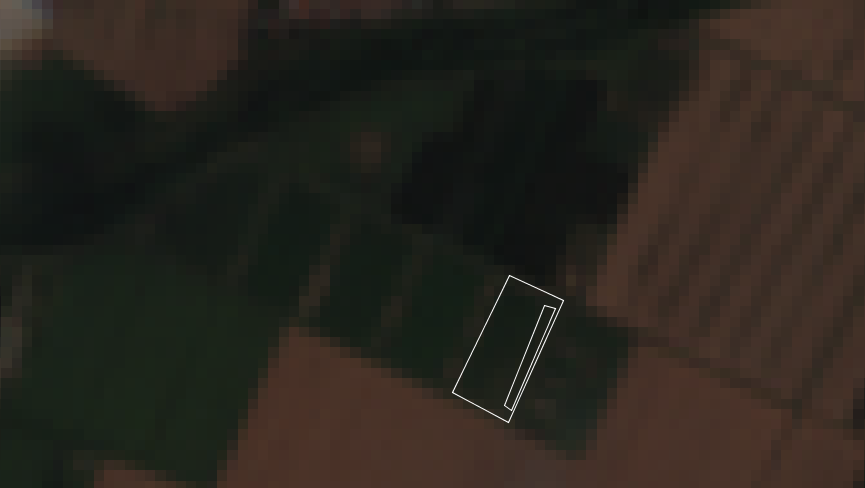
\includegraphics[width=.7\textwidth]{pics/roi.png}
  \caption[Region of Interest]{RGB-Sentinel-2-Aufnahme des zu untersuchenden Ackers. Die infizierten Flächen sind weiß umrandet. }
  \label{fig:roi}
\end{figure}
\noindent
Der infizierte Acker, der die Basis des Datensatzes bildet, befindet sich etwa $15$ km nordwestlich von Bologna in Norditalien (\ang{44;34;28,92} Nord, \ang{11;10;21,36} Ost). Das Feld hat eine Fläche von $7640,57$ m$^2$ und ist mit Sorghum bepflanzt. Mitarbeiter des CREA (Council for Agricultural Research and Economics) haben vor Ort am 12.07.2018 Befälle von Anthracnose und der bakteriellen Streifenkrankheit (med.: Xanthomonas translucens) diagnostiziert. Etwa die Hälfte der Pflanzen des Feldes sind betroffen. Dabei sind im östlichen Teil des Feldes (Abb. \ref{fig:roi}, innere Markierung) auf einer Fläche von $1043,22$ m$^2$ von etwa $60$ bis $70\%$ der Pflanzen befallen.

\section{Normalized Difference Vegetation Index}\label{sec:ndvi}

Es gibt eine starke Korrelation zwischen dem physiologischen Status einer Pflanze und deren Chlorophyllgehalt. Faktoren wie Krankheit, Dürre oder Umweltverschmutzung haben einen negativen Einfluss auf den Chlorophyllspiegel.\cite{ref:hendry} Messungen haben ergeben, dass es eine Verbindung zwischen dem Reflexionsgrad im nahen Infrarotbereich und im Rotbereich und dem Chlorophyllgehalt gibt. Das heißt, dass eine gesunde, adulte Pflanze im nahen Infrarotbereich stärker reflektiert als zum Beispiel eine pathologisch veränderte Pflanze. Jedoch bleibt die Reflexion im roten Lichtspektrum in beiden Fällen vergleichsweise schwach. Andere vegetationsfreie Oberflächen wie Acker, Straßen oder Wasser strahlen auch im nahen Infrarotbereich schwach zurück. Dadurch ergibt sich eine zerstörungsfreie Methode, mit einer Multispektralkamera die Vitalität ("`Grünheit"') einer oder mehrerer Pflanzen zu bestimmen.\cite{ref:anatoly} \\\\
Eine multispektralen Aufnahme kann mithilfe der Formel 
\begin{equation}\label{equation:ndvi}
	NDVI = \frac{Band_{NIR} - Band_{Red}} {Band_{NIR} + Band_{Red}}
\end{equation}
dazu genutzt werden, den \textit{Normalized Difference Vegetation Index} (NDVI) zu berechnen. Wobei $Band_{NIR}$ der nahe Infrarotbereich (Near Infrared) und $Band_{RED}$ der sichtbare rote Bereich des elektromagnetischen Spektrums ist. Der NDVI gibt quantifizierte Werte im Bereich von $-1$ bis $1$ zurück. Dabei deuten Werte, die kleiner als $0$ sind, auf Wasserobflächen hin. $0$ bedeutet keine Vegetation. Bei Werte nahe $0$ handelt es sich um spärliche oder ungesunde Vegetation. Das bedeutet je näher ein Wert an $1$ ist, desto dichter bewachsen und gesünder ist die beobachtete Vegetationsfläche.\cite{ref:nasa} Dass bei einem niedrigen, positiven NDVI nicht unterschieden werden kann, ob eine Fläche kaum bewachsen ist oder ungesunde Vegetation besitzt, kann hier vernachlässigt werden. Das Gebiet, das in dieser Arbeit untersucht wird, ist ein bewachsenes Feld, so kann man geringe Vegetation ausschließen. 

\section{Sentinel-2}\label{sec:sentinel2}

Die Sentinel-2-Satelliten sind eine von sechs Satellitenarten (Sentinel-1 bis -6) des Copernicus-Programms\footnote{Das Copernicus-Programm wurde von der Europäischen Union zur Erdbeobachtung ins Leben gerufen. Die gesammelten Daten werden für wissenschaftliche, wirtschaftliche und private Anwendungszwecke zur Verfügung gestellt.\cite{ref:copernicus}}, die zur Erdbeobachtung in einen 786 km hohen sonnensynchronen Orbit gebracht wurden. Die Instrumente der Sentinel-2-Satelliten können Aufnahmen in Bereichen des roten und nahen Infrarot- bis hin zum Kurzwelleninfrarotspektrums. Die Aufnahmen haben Gesamtgröße von $100*100$ km und je nach Band eine von Auflösung von 10m, 20m oder 60m (s. Tabelle \ref{tab:resolutions}).

\begin{table}[ht]
\centering
\begin{tabular}{c|c|c|c}
Bandnummer & Auflösung & Wellenlänge (nm) & Bandbreite (nm) \\
\hline
B1 & 60 & 443,9 & 27\\
B2 & 10 & 496,6 & 98\\
B3 & 10 & 560 & 45\\
B4 & 10 & 664,5 & 38\\
B5 & 20 & 703,9 & 19\\
B6 & 20 & 740,2 & 18\\
B7 & 20 & 782,5 & 28\\
B8 & 10 & 835,1 & 145\\
B8a & 20 & 864,8 & 33\\
B9 & 60 & 945 & 26\\
B10 & 60 & 1373,5 & 75\\
B11 & 20 & 1613,7 & 143\\
B12 & 20 & 2202,4 & 242\\
\end{tabular}
\caption{Räumliche und spektrale Auflösungen von Sentinel-2A\cite{ref:sentinel:radiores}}\label{tab:resolutions}
\end{table}
\noindent
Besonders wichtig sind die Bänder B4 (Rot) und B8 (Nahes Infrarot). Mit diesen Bändern kann der NDVI (s. Kapitel \ref{sec:ndvi}) berechnet werden.\cite{ref:sentinel:ndvi} Die Sentinel-2-Satelliten bieten mit $10*10$ m pro Pixel eine hohe räumliche Auflösung.\footnote{Im Vergleich hat zum Beispiel der Landsat-8-Satellit, dessen Daten ebenfalls frei verfügbar sind, eine relativ geringe Auflösung von $30*30$ m.\cite{ref:landsat}} Diese Eigenschaft ist wichtig, um eine mögliche Infizierung genau eingrenzen zu können.\\\\
Dabei ist es auch wichtig, dass die Satelliten regelmäßige Daten liefern können. Durch die gemeinsame Konstellation übertragen die Plattformen alle fünf Tage Daten über einen spezifischen Punkt auf der Erdoberfläche.\cite{ref:sentinel:resolutions} Damit ist gewährleistet, dass der Feldbesitzer ohne persönliche Inspektion ein bis zweimal in der Woche eine Gesundheitseinschätzung über seine Felder erhält.

\section{Das trainierbare Modell}\label{sec:maskrcnn}
In Kapitel \ref{sec:ndvi} und \ref{sec:sentinel2} wurde erklärt wie Daten über die möglichen Erkrankungen geliefert und verarbeitet werden können. Auf den zugrunde liegenden Bilddaten soll nun ein künstliches neuronales Netzwerk (KNN) trainiert werden. In diesem Kapitel wird darauf eingegangen, welche Anforderungen an das KNN gestellt werden, warum das Titel gebende Netz ausgewählt wurde und wie dieses funktioniert.

\subsection{Anforderungen}\label{sec:sub:requirements}
Das KNN muss in der Lage sein, wahrscheinliche Krankheiten in der zu untersuchenden Agrarfläche möglichst genau eingrenzen und klassifizieren zu können. Das ist besonders wichtig, wenn ein Feld von multiplen Krankheiten betroffen ist.\\\\
Es ist damit zu rechnen, dass Daten unter bewölkten Bedingungen aufgenommen werden. Nach starken Niederschlägen können Acker teils oder gänzlich überflutet sein.\cite{ref:root-rot} Das sorgt selbst unter wolkenfreien Bedingungen für einen niedrigen NDVI, obwohl die Nutzpflanzen gesund sind. Das neuronale Netz muss mit solchen \glqq Ausreißern\grqq{} umgehen können.
\\\\
Daraus ergeben sich folgende Kriterien für das neuronale Netzwerk:

\begin{itemize}
	\item Erkennung auf Pixelebene
	\item Robustheit
	\item Hohe Genauigkeit 
\end{itemize}

\subsection{Grundlagen}\label{sec:sub:basics}

\subsubsection{Vollständig vernetztes neuronales Netz}

\noindent
Künstliche neuronale Netze sind mathematische Modelle, die nach dem Vorbild von biologischen neuronalen Netzen gebildet worden sind. So ist ein KNN ebenfalls eine Verbindung von künstlichen Neuronen. Diese Neuronen sind in Schichten angeordnet und jede die Neuronen einer Schicht sind mit den Neuronen nächsten bzw. letzten Schicht verbunden. Zwischen der ersten und der letzten sog. Ausgangsschicht existieren $n$ versteckte Schichten (engl.: hidden layers). 

\begin{figure}[ht]
  \centering
  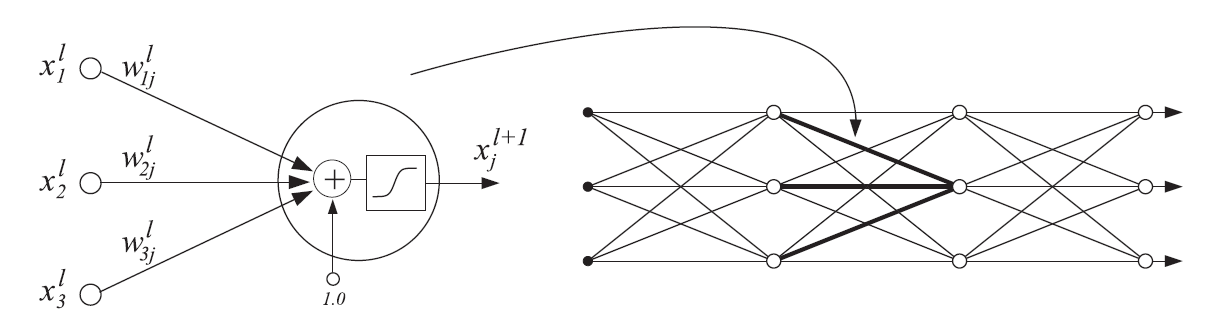
\includegraphics[width=0.8\textwidth]{pics/neural-net.PNG}
  \caption[Künstliches neuronales Netz]{Künstliches neuronales Netz\cite{ref:verrelst}}
  \label{fig:ann}
\end{figure}
\noindent
Ein Neuron besitzt mehrere Eingangsverbindungen (Gewichte) und ein Ausgangsneuron. Ob ein Neuron "`feuert"', wird durch eine lineare oder nicht-lineare Aktivierungsfunktion bestimmt. Die Eingangsgewichte sind veränderbare Werte, die je nach Höhe einen starken oder niedrigen Einfluss auf die Aktivierungsfunktion haben.
\begin{equation}\label{equ:neuron}
x^{l+1}_{j}=f(\sum\nolimits_i w^l_{ij}x^l_i + w^l_{bj})
\end{equation}
beschreibt das Neuron $j$ in Schicht $l+1$, wobei
\begin{itemize}
	\item $w^l_{ij}$ die Gewichte sind, die Neuron $i$ in Schicht $l$ mit Neuron $j$ verbinden.
	\item $w^l_{bj}$ der Biasterm des $j$-ten Neurons in Schicht $l$ ist.
	\item $f$ die Aktivierungsfunktion ist.\cite{ref:verrelst}
\end{itemize} 

\subsubsection{Convolutional Neural Networks}\label{sec:sub:sub:cnn}
\begin{figure}[ht]
  \centering
  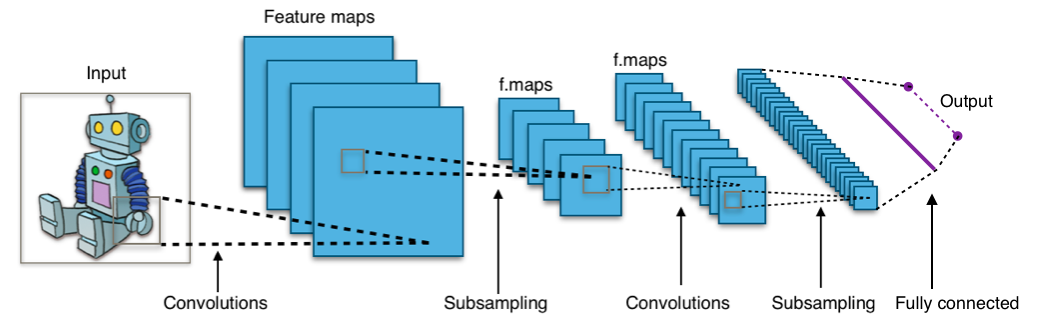
\includegraphics[width=0.95\textwidth]{pics/cnn.png}
  \caption[CNN]{Architektur eines Convolutional Neural Network\cite{ref:cnn-architecture}}
  \label{fig:cnn-architecture}
\end{figure}

\noindent 
\textit{Convolutional Neural Networks} (CNN, dt.: faltendes neuronales Netzwerk) sind Kategorien von neuronalen Netzen, die besonders in der \textit{Computer Vision} Anwendung finden. In der ersten Schicht werden mehrere Merkmale (engl.: features) durch Filter extrahiert und in separate sog. \textit{Feature Maps} abgelegt, um größere Abstraktionsebenen zu erreichen. Diese Filter sind mathematisch mit Faltungen (engl.: convolutions) zu vergleichen und geben dem Netz den Namen. 
\\\\
Die Dimensionen der Feature Maps werden in einem Poolingschritt\footnote{Es gibt verschiedene Arten von Pooling (Max, Average, Sum, ...). Dabei wird die $m*m$ px große Feature Map in sich angrenzende $n*n$ px große Felder eingeteilt ($n<m$). Im Falle von Max-Pooling wird der höchste Wert aus dem Feld übernommen.} (oder auch \textit{subsampling}) reduziert. Dadurch bleiben nur relevante Informationen erhalten und das CNN wird bis zu einem gewissen Grad robust gegenüber Translationen und Rotationen. In der Regel werden die Faltungen und das das Pooling zwei Mal durchgeführt, wie es in Abb. \ref{fig:cnn-architecture} abgebildet ist.
\\\\
Nach der Merkmalextraktion werden die Feature Maps zur Klassifikation in eine eindimensionale Schichten geglättet. Die folgenden Schichten bis zur Ausgangsschicht sind vollständig vernetzt.


\subsection{Mask R-CNN}\label{sec:sub:mask-rcnn}

Im Rahmen dieser Arbeit wird das \textit{Mask Region-based Convolutional Neural Network} untersucht. Mask R-CNN ist eine von Facebook AI Research (FAIR) entwickelte Erweiterung des \textit{Faster R-CNN} und kann verschiedene Instanzen einer Klasse in einem Bild von einander trennen. Dazu muss zuerst die Begriffe der Instanzsegmentierung definiert werden.
\\\\
\begin{figure}[ht]
  \centering
  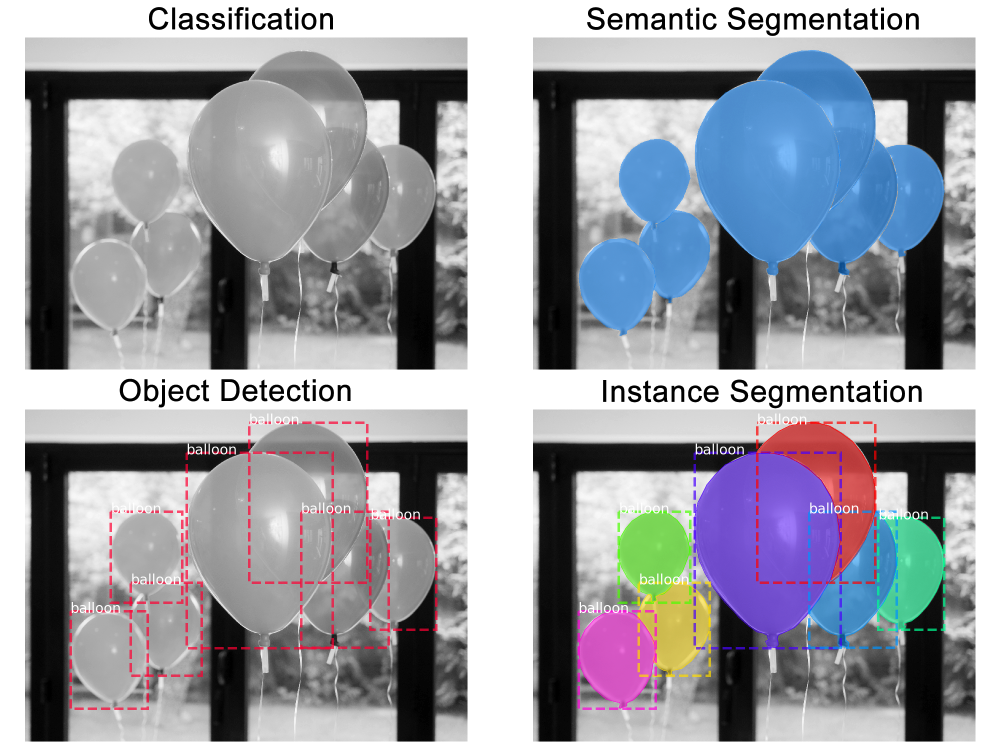
\includegraphics[width=0.8\textwidth]{pics/instance-segmentation.png}
  \caption[Instanzsegmentierung]{Unterschied Klassifizierung / semantische Segmentierung / Objekterkennung / Instanzsegmentierung\cite{ref:matterport:maskrcnn}}
  \label{fig:instance-segmentation}
\end{figure}
\noindent
Einfache Klassifizierung (engl.: classification) ordnet Bilder als Ganzes einer Klasse zu. \textit{Semantische Segmentierung} (engl.: semantic segmentation) beschreibt die Klassifizierung auf Pixelebene. Es wird erkannt zu welcher Klasse eine Menge von Pixeln gehören, aber es wird nicht zwischen einzelnen Objekten unterschieden. \textit{Objekterkennung} (engl.: object detection) entdeckt und lokalisiert unterschiedliche Objekte, indem es eine Bounding Box um jedes erkannte Objekt zieht. Jedoch fehlt hier die pixelgenaue Abgrenzung einzelner Objektinstanzen. \text{Instanzsegmentierung} (engl.: instance segmentation) kombiniert \textit{Objekterkennung} und \textit{semantische Segmentierung} und ist so in der Lage zwischen einzelnen Objekten zu unterscheiden und ihnen entsprechende Pixel zuzuordnen (s. Abb. \ref{fig:instance-segmentation}) und ist eine der größten Herausforderungen in der Bildverarbeitung.\cite{ref:maskrcnn}
\\\\
\begin{figure}[ht]
  \centering
  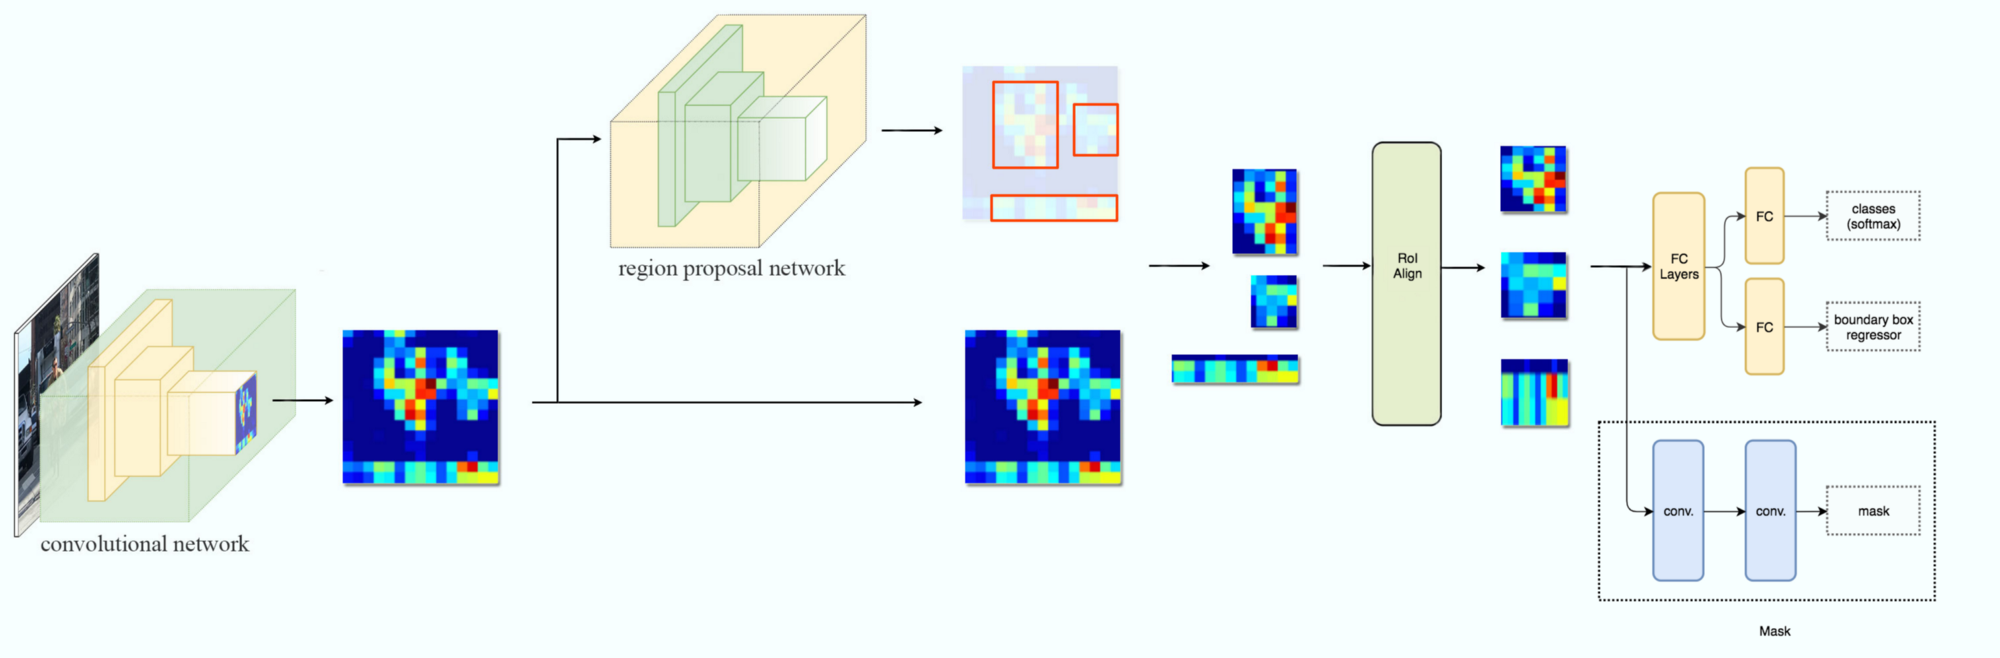
\includegraphics[width=\textwidth]{pics/maskrcnn-archtecture.PNG}
  \caption[Mask R-CNN-Architektur]{Mask R-CNN-Architektur\cite{ref:mask-rcnn-architecture}}
  \label{fig:maskrcnn-architecture}
\end{figure}
\noindent
Mask R-CNN ist wie Faster R-CNN in zwei Segmente eingeteilt. In dem ersten Segment, dem \textit{Region Proposal Network} (oder auch RPN), werden mehrere Rahmen (engl.: Bounding Boxes) innerhalb eines Bildes vorgeschlagen, die interessante Objekte beinhalten könnten. Das RPN erzeugt Rechtecke - sog. Anker (engl.: Anchors) - von unterschiedlichen Größen und Bildverhältnissen, die sich über die Bildregion verteilen und sich überlappen. Für jeden Anker wird eine Ankerklasse und eine Bounding-Box-Verfeinerung ausgegeben. Die Klasse unterscheidet Vordergrund und Hintergrund, wobei eine Bounding-Box mit Vordergrundklassifizierung als potentielle Objekterkennung gewertet wird. Ein Anker ist möglicherweise nicht genau über ein Objekt zentriert. Die Verfeinerung ist eine geschätze Veränderung des Ankers in Position, Höhe und Größe, um besser das Objekt umrahmen zu können. Wenn mehrere Anker sich zu sehr überschneiden, wird der Anker mit der höchsten Wahrscheinlichkeit ein Objekt zu beinhalten übernommen und der restlichen Anker werden verworfen.\footnote{Diese Methode wird \textit{Non-max suppression} genannt.}\cite{ref:matterport:maskrcnn}\cite{ref:faster-r-cnn} Die vorgeschlagene Regionen, die einzeln von CNNs bewertet werden, ist der Kernansatz von R-CNN. Das RPN wurde identisch von Faster R-CNN für Mask R-CNN übernommen.\cite{ref:maskrcnn} 
\\\\
\begin{figure}[ht]
  \centering
  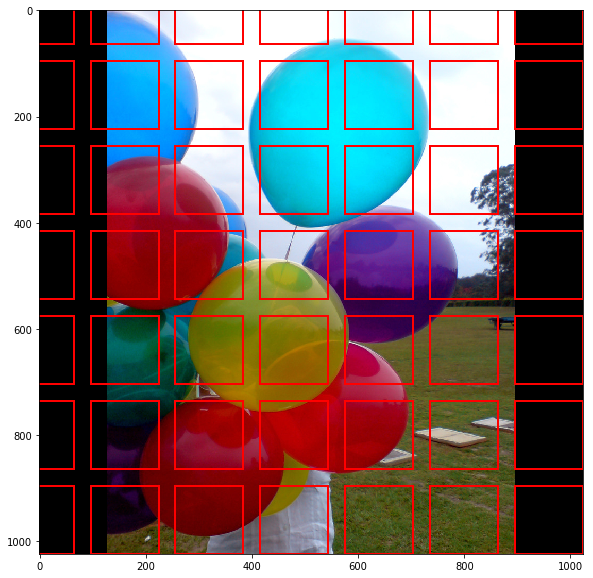
\includegraphics[width=.45\textwidth]{pics/rpn-anchors.png}
  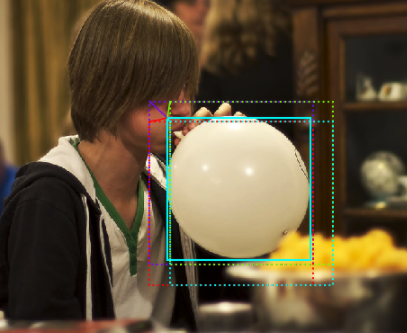
\includegraphics[width=.45\textwidth]{pics/rpn-refinement.png}
  \caption[RPN-Anker]{Links: Vereinfachte Darstellung von Ankern über ein Bild\cite{ref:matterport:maskrcnn} / Rechts: Drei Anker (gepunktet), die das das gleiche Objekt umschließen und die Verfeinerung (durchgezogen), die auf diese angewendet wird, um das Objekt genauer einzugrenzen\cite{ref:matterport:maskrcnn}}
  \label{fig:rpn}
\end{figure}
\noindent
Im zweiten Segment werden aus den Regionen \textit{Bounding Boxes} (dt.: Rahmen) und Masken generiert und klassifiziert. Die Rahmen haben verschiedene Größen und können Probleme bei der Klassifizierung verursachen. Daher werden die Rahmen auf eine kleine Feature Map gleicher Größe (z.B. $7*7$ px) reduziert. Die Authoren von \cite{ref:maskrcnn} schlagen eine Methode namens \textit{RoI-Align} vor, bei der Proben aus der Feature Map entnommen werden und eine bilineare Interpolation angewendet wird. In dem bei Faster R-CNN angewandten Verfahren \textit{RoI-Pooling} entstehen durch Quantisierung Informationsverluste und räumliche Abweichungen zwischen Bounding Box und Feature Map, was negative Auswirkungen auf die Maskengenerierung haben kann.\cite{ref:maskrcnn}
\\\\
\begin{figure}[ht]
  \centering
  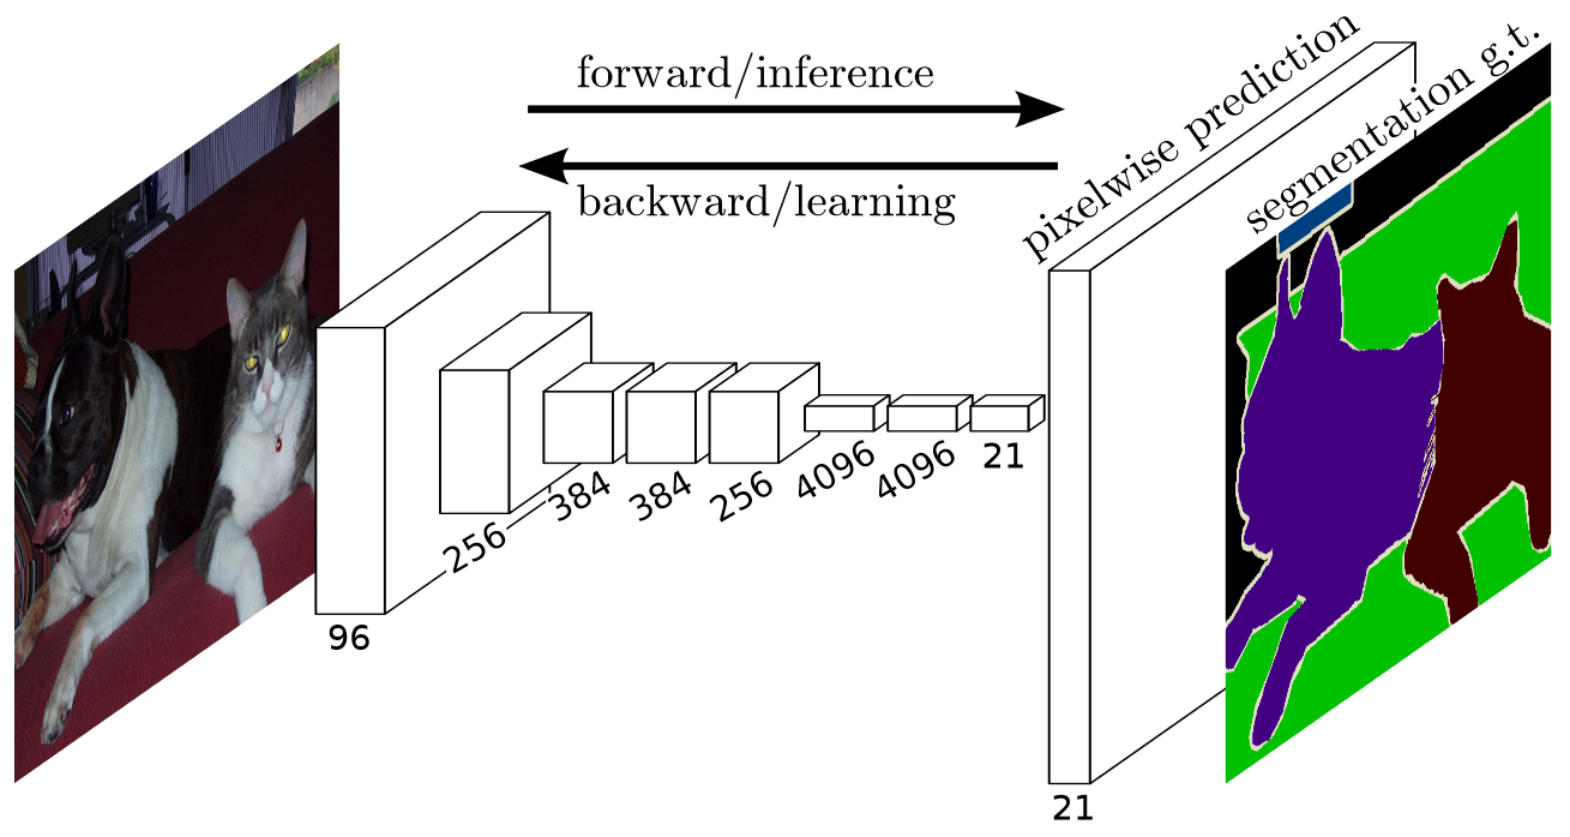
\includegraphics[width=0.90\textwidth]{pics/fcn-architecture.PNG}
  \caption[FCN-Architektur]{FCN-Architektur\cite{ref:mask-rcnn-architecture}}
  \label{fig:fcn-architecture}
\end{figure}
\noindent
Die oberen vollständig vernetzten Schichten (\textit{FC Layers} in Abb. \ref{fig:maskrcnn-architecture}) klassifizieren die Regionen und die Bounding Boxes berechnet. Dieser Zweig ist für die Objekterkennung wichtig und noch mit Faster R-CNN gemeinsam. 
\\\\
Gleichzeitig werden in einem parallelen Zweig je Bounding Box $k$ $m*n$ große Masken zur semantischen Segmentierung erzeugt, wobei $k$ die Anzahl der Klassen ist.  Anders als in dem ersten Zweig des zweiten Segmentes werden die Masken durch \textit{fully convolutional networks} (FCN, dt.: vollständig faltende Netzwerke) prognostiziert. Diese bestehen nur aus faltenden Schichten, wie sie in Kapitel \ref{sec:sub:sub:cnn} beschrieben sind. Eine Maske ist eine räumliche Kodierung eines Objektes und daher ist es wichtig räumliche Informationen beizubehalten. Diese können durch die Pixel-zu-Pixel-Übereinstimmung extrahiert werden, welche sonst durch vollständig vernetzter Schichten verloren gehen. Diese geben einen Vektor ohne räumliche Dimensionen aus.\cite{ref:maskrcnn}
\\\\
\begin{figure}[ht]
  \centering
  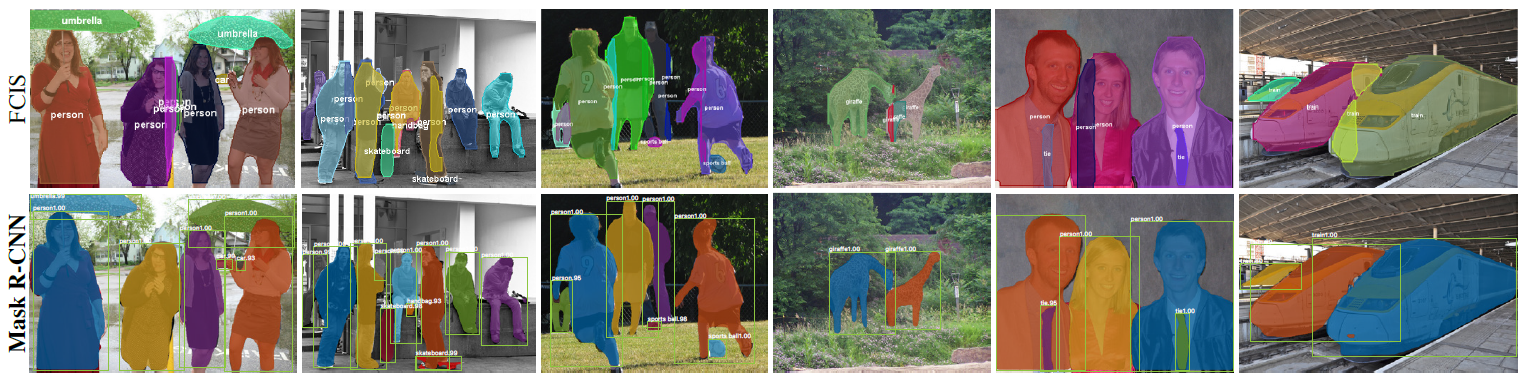
\includegraphics[width=\textwidth, height=5cm]{pics/mrcnn-vs-fcis.PNG}
  \caption[Mask R-CNN vs. FCIS]{Bei FCIS entstehen Artefakte, wenn Objekte sich in einem Bild überlappen.\cite{ref:maskrcnn}}
  \label{fig:maskvsfcis}
\end{figure}
\begin{table}[ht]
  \centering
  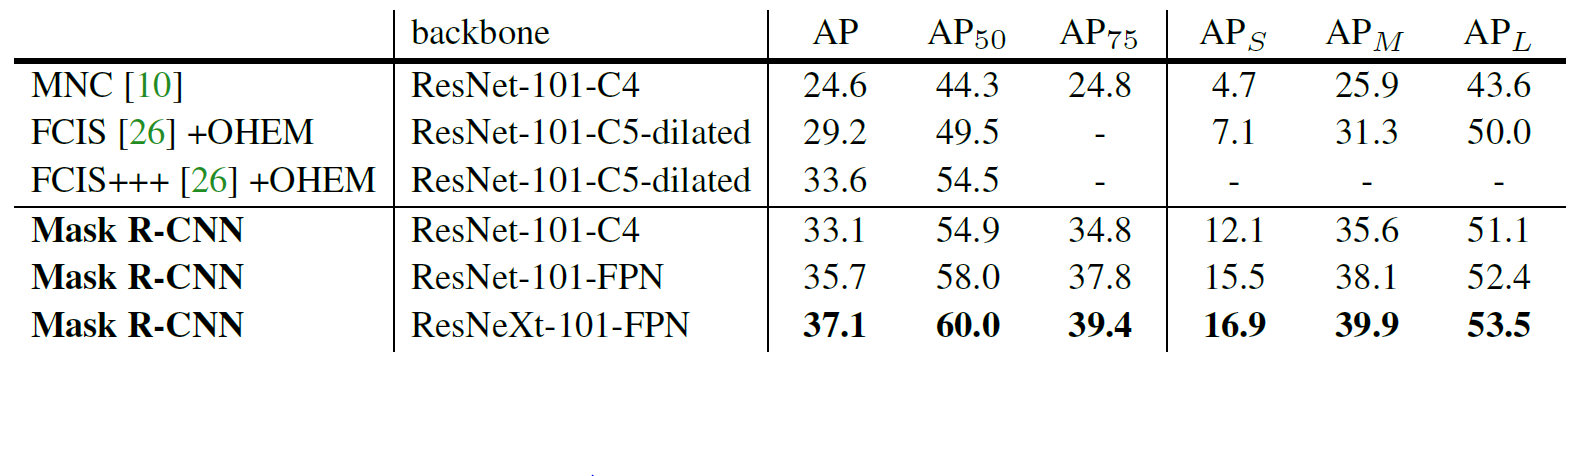
\includegraphics[width=\textwidth]{pics/mrcnn-vs-fcis-vs-mnc.PNG}
  \caption[Mask R-CNN im Vergleich]{Instance segmentation \textit{mask} AP auf COCO \textit{test-dev}. MNC und FCIS sind Sieger der COCO 2015 und 2016 Challenge. Mask R-CNN erzielt deutlich bessere Ergebnisse als die komplexere FCIS+++.\cite{ref:maskrcnn}}
  \label{tab:maskvsfcisvsmnc}
\end{table}
\noindent
In \cite{ref:maskrcnn} wird Mask R-CNN mit den \textit{COCO challenge}-Gewinnern\footnote{COCO (Common Objects in Context, dt.: Gewöhnliche Objekte im Kontext) enthält einen Datensatz von über 200000 Bildern in über 80 Kategorien. Der Datensatz ist eine oft genutzte Basis, um Objekterkennungstechniken zu evaluieren und zu bewerten.\cite{ref:coco}} der Jahre 2015 und 2016 verglichen. Der Vergleich zeigt, dass Mask R-CNN in der Challenge bessere Werte erzielt als die Konkurenten (s. Tab. \. Desweiteren fällt \textit{fully convolutional instance segmentation} (FCIS, dt.: vollständig faltende Instanzsegmentierung) auf, wenn es mit überlappenden Objekten konfrontiert wird. Dort erzeugt es Artefakte, welche durch Mask R-CNN nicht entstehen (s. Abb. \ref{fig:maskvsfcis}). Durch diese Gegenüberstellungen wird gezeigt, dass Mask R-CNN alle aufgeführten Anforderungen erzielt. Es erkennt Klasseninstanzen auf Pixelebene und weist eine hohe Robustheit auf. Auch die Genauigkeit hebt sich beim direkten Vergleich ab. Aus diesen Gründen wurde Mask R-CNN im Rahmen diese Arbeit ausgewählt.

\section{Evaluation des Modells}\label{sec:map}

Jetzt wo gezeigt wurde, welches Modell in dieser Arbeit genutzt wird, fehlt eine Möglichkeit ein trainiertes Modell zu bewerten. \textit{Mean average precision} (oder auch mAP) ist eine Metrik, um die Genauigkeit einer Instanzsegmentierung zu messen.\footnote{mAP ist nicht nur auf Instanzsegmentierung limitiert, sondern wird zum Beispiel auch als Metrik in der Objekterkennung genutzt.} Aber bevor die erklärt werden können, muss noch die Begriffe \textit{Precision}, \textit{Recall} und \textit{Intersection over Union} eingegangen werden. 


\subsection{Intersection over Union}

\textit{Intersection over Union} (oder auch IoU, dt: Schnitt über Vereinigung) ist eine wichtige Metrik für die semantische Segmentierung. Sie vergleicht die vorhergesagte Maske mit der Grundwahrheit\footnote{Die Grundwahrheit (engl.: ground truth) ist hier die binäre Maske, die die infizierte Fläche repräsentiert.}, um zu messen wie gut die Vorhersage mit der Grundwahrheit übereineinstimmt.\cite{ref:map}

\begin{equation}\label{equation:recall}
  IoU = \frac{Grundwahrheit\cap Vorhersage}{Grundwahrheit\cup Vorhersage}
\end{equation}
\noindent
Die Schnittmenge beinhaltet alle Pixel, die sich in der Grundwahrheit als auch in der vorhergesagten Maske befinden. Pixel, die sich in der Grundwahrheit und in der Vorhersage befinden, werden von der Vereinigung zusammengefasst. 
\\\\
\begin{figure}[ht]
  \centering
  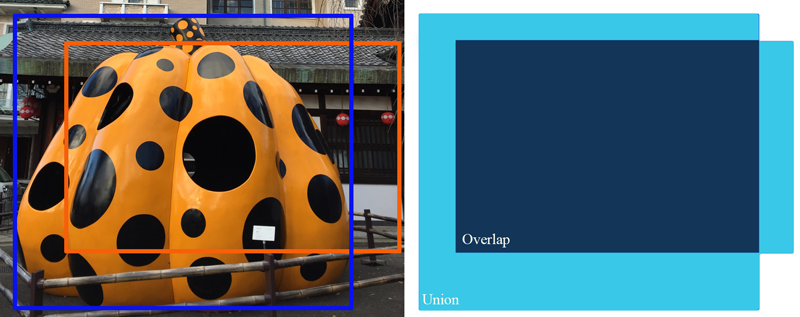
\includegraphics[width=\textwidth]{pics/iou.PNG}
  \caption[IoU]{Beispiel Intersection over Union, Grundwahrheit in blau, Vorhersage in rot\cite{ref:map}}
  \label{fig:iou}
\end{figure}
\noindent
In der semantischen Segmentierung wird für jede Klasse ein unterschiedlicher IoU-Wert berechnet und dann wird der Mittelwert aus diesen Werten ermittelt, um einen globalen Messwert zu haben. In der Instanzsegmenierung wird für jede einzelne Objektinstanz mittels Instanzgrundwahrheit und Instanzvorhersage ein separater IoU-Wert berechnet. Wenn ein bestimmter Grenzwert überschritten wird, gilt diese Instanz als tatsächlich richtige Erkennung.\cite{ref:jordan}

\subsection{Precision und Recall}

\textit{Precision} (oder auch Falsch-Positiv-Rate) sagt aus mit welcher Wahrscheinlichkeit eine Vorhersage korrekt ist. Diese Metrik wird durch die Formel 
\begin{equation}\label{equation:precision}
  Precison = \frac{RP}{RP + FP}
\end{equation}
berechnet, wobei $RP$ (Richtig-Positiv) die Anzahl der richtigen Erkennungen und $FP$ (Falsch-Positiv) die Anzahl der falschen Erkennungen sei.\cite{ref:map} \textit{Precision} ist also der Anteil von tätsächlich richtigen Erkennungen in Relation zu allen Erkennungen. In Bezug auf Instanzsegmentierung wird die Frage beantwortet, wie viele der erkannten Objekte in einem Bild tatsächlich eine passende Grundwahrheitüberschneidung und eine IoU-Grenzwertüberschreitung haben.\cite{ref:jordan}
\\\\
\textit{Recall} (oder auch Falsch-Negativ-Rate) misst die Wahrscheinlichkeit, dass alle tatsächlich wahren Detektionen korrekt erkannt wurden. Diese Metrik wird durch die Formel 
\begin{equation}\label{equation:recall}
  Precison = \frac{RP}{RP + FN}
\end{equation}
berechnet, wobei $RP$ (Richtig-Positiv) die Anzahl der richtigen Erkennungen und $FN$ (Falsch-Negativ) die Anzahl der Objekte, die fälschlicherweise nicht erkannt wurden, sei. \textit{Recall} ist also der Anteil von tätsächlich richtigen Erkennungen in Relation zu allen Objekten im Datensatz.\cite{ref:map} In Bezug auf Instanzsegmentierung wird die Frage beantwortet, wie viele der Objekte mit Grundwahrheit in einem Bild als tatsächlich richtig erkannt werden und eine IoU-Grenzwertüberschreitung haben.\cite{ref:jordan}

\subsection{Average Precision}

\begin{figure}[ht]
  \centering
  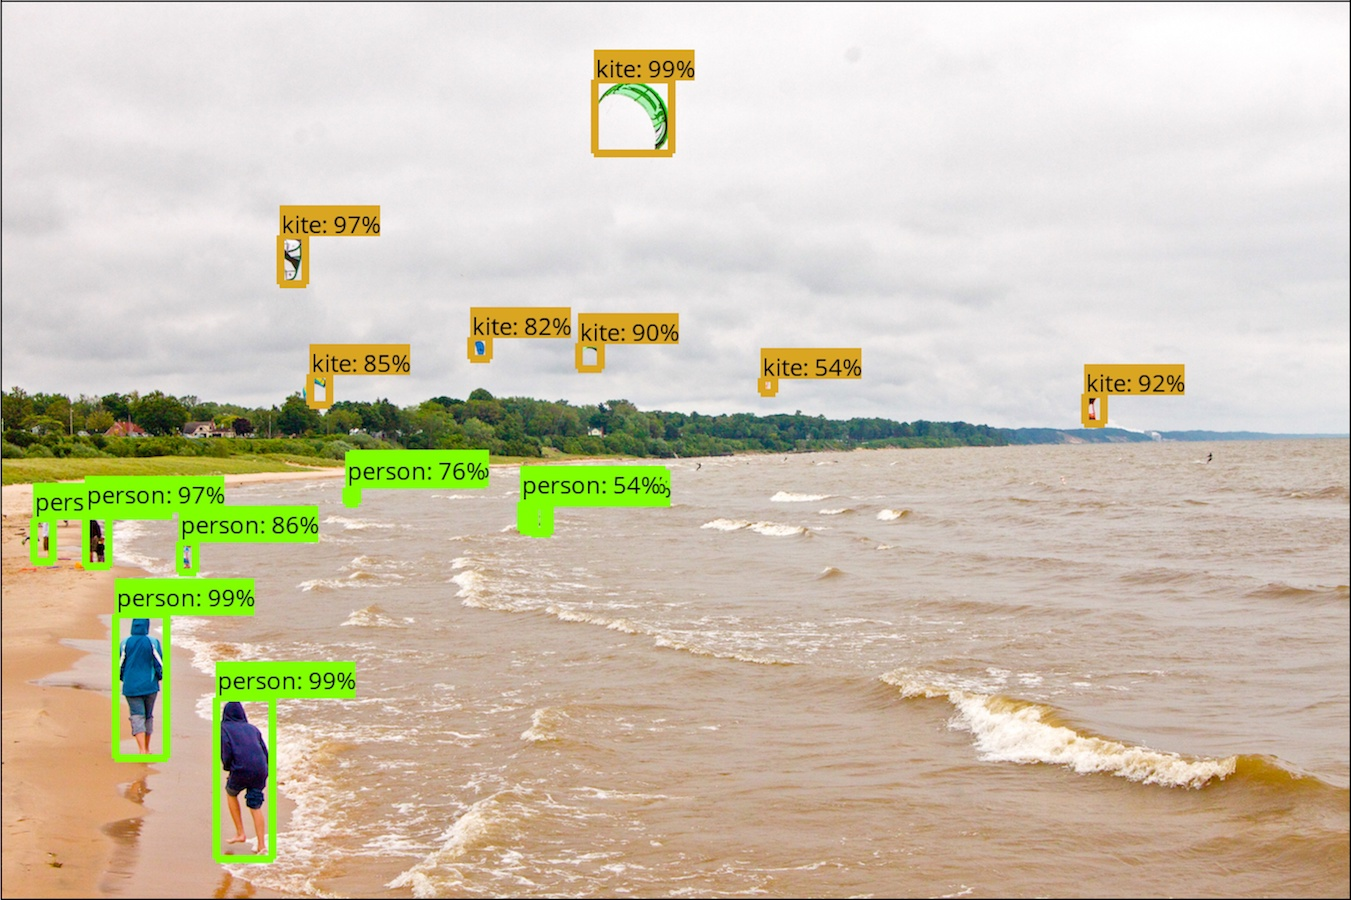
\includegraphics[height=5cm]{pics/kites.jpg}
  \hspace{.5cm}
  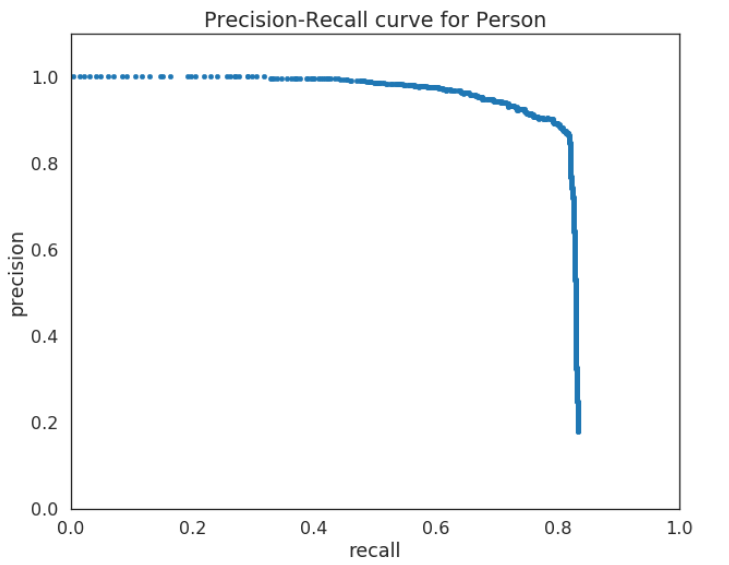
\includegraphics[height=5cm]{pics/precision-recall-kurve.png}
  \caption[Precision-Recall-Kurve]{Links: Beispielbild mit multiplen Detektionen und Klassen\cite{ref:arlen}\\Rechts: Beispiel Precision-Recall-Kurve für die Klasse ``Person''\cite{ref:huang}}
  \label{fig:precision-recall}
\end{figure}
\noindent
Ein \textit{Precision}- und \textit{Recall}-Wert bezieht sich jeweils auf eine detektierte Objektinstanz einer Klasse. Bei mehreren detektierten Objekte einer Klasse in einem Bild können diese in einer Precision-Recall-Kurve visualisiert werden (s. Abb. \ref{fig:precision-recall}). \textit{Average Precision} (oder auch AP) fasst die Form der Kurve zu einem Wert zusammen, indem es den Durchschnitt der \textit{Precision}-Werte an elf \textit{Recall}-Werten $[0, 0.1, \dots, 1]$ berechnet: 

\begin{equation}\label{equation:ap}
  AP = \frac{1}{11} \sum_{r \in \{0, 0.1, \dots, 1\}}  p_{interp}(r)
\end{equation}
\noindent
Ein \textit{Precision}-Wert $p$ an der \textit{Recall}-Stelle $r$ wird interpoliert, indem der Maximumwert übernommen an der \textit{Recall}-Stelle $\tilde{r}\ge r$ wird:

\begin{equation}\label{equation:pinterp}
  p_{interp}(r) = \max_{\tilde{r}:\tilde{r}\ge r} p (\tilde{r})
\end{equation}
\noindent
wobei $p(\tilde{r})$ der \textit{Precision}-Wert $p$ an der \textit{Recall}-Stelle $\tilde{r}$ sei. Die Interpolation reduziert den Einfluss kleiner, lokaler Unebenheiten in der Kurve.\cite{ref:huang}

\subsection{Mean Average Precision}

\textit{Mean Average Precision} ist der Durschschnitt aller \textit{Average Precision}-Werte jeder Klasse in jedem Element eines (Sub-)Datensatzes.\footnote{\textit{mAP} wird oft nur \textit{AP} genannt.} \textit{mAP} wird zum Beispiel auch in der COCO- oder PASCAL-VOC-Challenge benutzt, um die Resultate der Challenge-Teilnehmer zu bewerten (s. Tabelle \ref{tab:maskvsfcisvsmnc}). Aber hier kann es zu Unterschieden kommen, wie der \textit{mAP} berechnet wird. So ist es bei der COCO-Challenge der durchschnittliche \textit{mAP} über verschiedene \textit{IoU}-Grenzwerte. Hier wird jeweils ein \text{mAP} an zehn verschiedenen \textit{IoU}-Werten $[0.5, 0.55, \dots, 0.95]$ berechnet und aus den Ergebnissen wird der Durchschnitt ermittelt.\cite{ref:coco:eval} In dieser Arbeit wird stets $IoU=0.5$ als Grenzwert benutzt, um die Auswertung einfach zu halten.
\chapter{Overfitting}\label{chap:overfitting}

\section{Begriffserklärung}\label{sec:what-is-overfitting}

Genaue Daten über Krankheitsbefälle im Agrarsektor sind rar, da diese in der Regel nicht öffentlich zugänglich sind.\footnote{Datenschutz kann ein Grund dafür sein.}  Daher musste mit \textit{Overfitting} gerechnet werden. Das künstliche neurale Netzwerk soll daraufhin trainiert werden, dass es möglichst alle Befälle, die untersucht werden, erkennt. Dafür wird es im ersten Schritt mit einem Trainingsdatensatz trainiert. Im folgenden Schritt mit einem kleineren Validierungsdatensatz überprüft, wie gut das Netz trainiert wird. Overfitting tritt auf, wenn das Netz auf die Daten aus dem Trainingsdatensatz mit sehr hoher Erfolgsquote erkennt, jedoch vergleichsweise schlechte Ergebnisse bei der Validierung bzw. bei unbekannten Daten erzielt. 
\\\\
\begin{figure}[ht]
  \centering
  
\includegraphics[height=2.5cm]{pics/mask.png}
  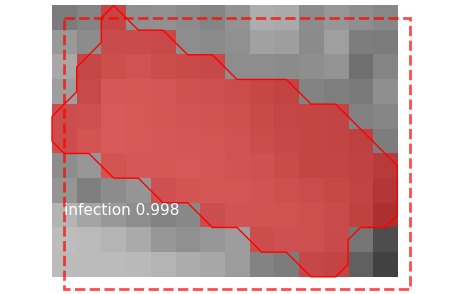
\includegraphics[height=2.5cm]{pics/pred.png}
  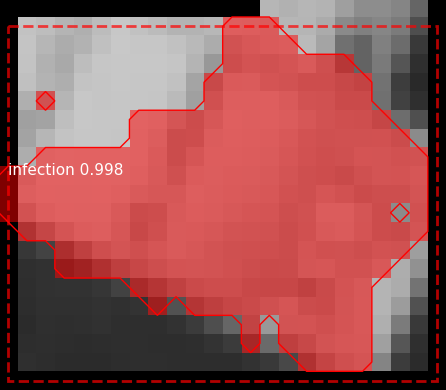
\includegraphics[height=2.5cm]{pics/bad-pred.png}
  \caption[Beispiel Overfitting]{V.l.n.r. Bild von infizierter Agrarfläche aus Trainingsdatensatz / Binärmaske der inifizierten Region, wird gemeinsam mit dem linken Bild zum Training in das KNN gespeist / Selbiges Bild, Ergebnis nach Trainingsdurchlauf, prognostizierte Ergebnisfläche in rot / Bild der selben Fläche, was nicht aus dem Trainingsdatensatz stammt, prognostizierte Ergebnisfläche in rot}
  \label{fig:example-overfitting}
\end{figure}
\noindent
\todo{Erwähnen, dass Mask RCNN Bild und Masken für Training benötigt.}
In Abb. \ref{fig:example-overfitting} ist ein Beispiel wie Overfitting sich auswirken kann. Die linken zwei Bilder sind ein exemplarischer Auszug aus dem Trainingsdatensatz. Einmal eine visuelle Repräsentation der NDVI-Werte der infizierten Agrarfläche und die Binärmaske, welche die infizierte Fläche markiert. Das selbe Bild wurde nach einem erfolgreichen Trainingsdurchlauf der Mask R-CNN-Implementierung übergeben und es hat den erkrankten Bereich nahezu perfekt erkannt. Das vierte Bild zeigt zentriert das selbe Feld. Jedoch ist der Ausschnitt größer, rotiert und die Aufnahme stammt von einem anderen Datum.\todo{Genaues Datum nötig?} Der Prognose zur Folge ist die Infizierung auf die benachbarten Felder übergesprungen, was nicht der Wahrheit entspricht. Overfitting ist ein bekanntes Problem im Bereich des maschinellen Lernens und es existieren multiple Methoden, um dem entgegenzuwirken.
\chapter{Konzept und Implementierung}\label{chap:concept}

\section{Konzept}\label{sec:concept}

Das Programmablauf wird in einzelne Schritte unterteilt, auf die in den nächsten Kapiteln näher eingegangen werden.
\\\\
\begin{figure}[ht]
  \centering
  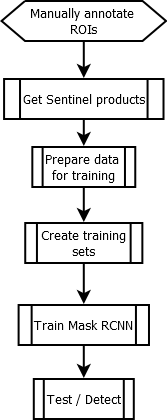
\includegraphics[width=.2\textwidth]{pics/overview.PNG}
  \caption{Gesamtablauf der Anwendung}
  \label{fig:overview}
\end{figure}
Zuerst müssen die Daten für das Training bzw. für die Erkennung manuell annotiert werden. Diese Metadaten werden dann genutzt, um automatisch Sentinelprodukte\footnote{Aufnahmenpakete der Sentinel-Plattformen werden als Produkte bezeichnet.} mittels einer API, die von der Copernicus zur Verfügung gestellt wird, herunterzuladen. Aus den Produkten werden die relevanten Bänder extrahiert und unter anderem die jeweiligen NDVI-Werte berechnet. Nachdem die Produkte für das Training vorbereitet wurden, werden die Daten in ein Trainings- und in ein Validierungsdatensatz aufgeteilt. Der folgende Trainingsprozess basiert auf diesen Datensätzen. Sobald das Training abgeschlossen ist, kann die Performanz des Modells getestet werden. 

\section{Annotation}\label{sec:annotation}

Zu Beginn werden die Regionen, die entweder für das Training benutzt oder überprüft werden, manuell erfasst. Vorrausgesetzte Informationen sind
\begin{itemize}
	\item Geografische Koordinaten,
	\item Zeitraum des Befalls und
	\item Bezeichnung der Infektion.
\end{itemize}
Als Format dieser Informationen dient \textit{GeoJSON}\footnote{GeoJSON ist eine Erweiterung des JSON-Format und beschreibt geografische Daten und Geometrien. GeoJSON wird durch den RFC7946-Standard definiert.}. GeoJSON enthält nicht nur geografische Daten, sondern ist auch um benutzerdefinierte Eigenschaften (\texttt{properties}) erweiterbar. Die Annotationen sind also GeoJSON-Features, die ein geografisches Polygon und Metadaten enthalten.

\begin{lstlisting}[language=json,caption={Annotation},captionpos=b]
{
  "type": "Feature",
  "properties": {
    "disease": 1,
    "from": "2018-07-12T13:00:00Z-7DAYS",
    "to": "2018-07-12T13:00:00Z+7DAYS"
  },
  "geometry": {
    "type": "Polygon",
    "coordinates": [[[11.171988617177981,44.574291380353003],
       [11.1726616444942,44.574017992242283],
       [11.17338129910439,44.575068359984279],
       [11.17273129334275,44.575299863118993],
       [11.171988617177981,44.574291380353003]]]
  }
}
\end{lstlisting}
\noindent
\texttt{properties.disease} enthält die eindeutige, nummerische Repräsentation der Klasse bzw. Krankheit, die in dieser Region enthalten ist. Die Zuordnung der nummerischen Werte und des textuellen Bezeichners werden in einer separaten JSON als Schlüssel-Wert-Paare konfiguiert, wobei der Schlüssel nummerisch und der Wert textuell ist. Hier ist, darauf zu achten, dass der Schlüssel $\ge1$ ist, da $0$ der implizite Schlüssel der Mask R-CNN-Implementierung für den Hintergrund ist. Diese Eigenschaft ist nur für das Training von Relevanz.
\\\\
\texttt{properties.from} und \texttt{properties.to} sind jeweils Start- und Endzeitpunkt, in dem nach verfügbaren Sentinelprodukten gesucht werden soll. Das Format der jeweiligen Eigenschaften kann eine der folgenden Formen haben\footnote{Die Formate basieren auf der \texttt{sentinelsat}-Version 0.12.2.}:
\begin{itemize}
	\item \texttt{yyyyMMdd}
	\item \texttt{yyyy-MM-ddThh:mm:ss.SSSZ} (ISO-8601)
	\item \texttt{yyyy-MM-ddThh:mm:ssZ}
	\item \texttt{NOW}
	\item \texttt{NOW-<n>DAY(S)} (oder \texttt{HOUR(S)}, \texttt{MONTH(S)}, usw.)
	\item \texttt{NOW+<n>DAY(S)}
	\item \texttt{yyyy-MM-ddThh:mm:ssZ-<n>DAY(S)}
	\item \texttt{NOW/DAY} (oder \texttt{HOUR}, \texttt{MONTH} usw.) - Der Wert wird auf den jeweiligen Typ (z.B. auf den Tag) gerundet.
\end{itemize}
\noindent
Es ist angebracht einen Zeitraum von mehreren Tagen bzw. Wochen zu wählen, da die Sentinel-2-Satelliten keine täglichen Daten liefern und weil eine Infektion typischerweise über einen längeren Zeitraum vorherrscht. Die Zeitspanne ist von der Krankheit abhängig. Hier wurden eine Woche vor und nach dem Aufnahmezeitpunkt genutzt, um nach Produkten zu suchen.

\section{Suche nach Sentinelprodukte}

\begin{figure}[ht]
  \centering
  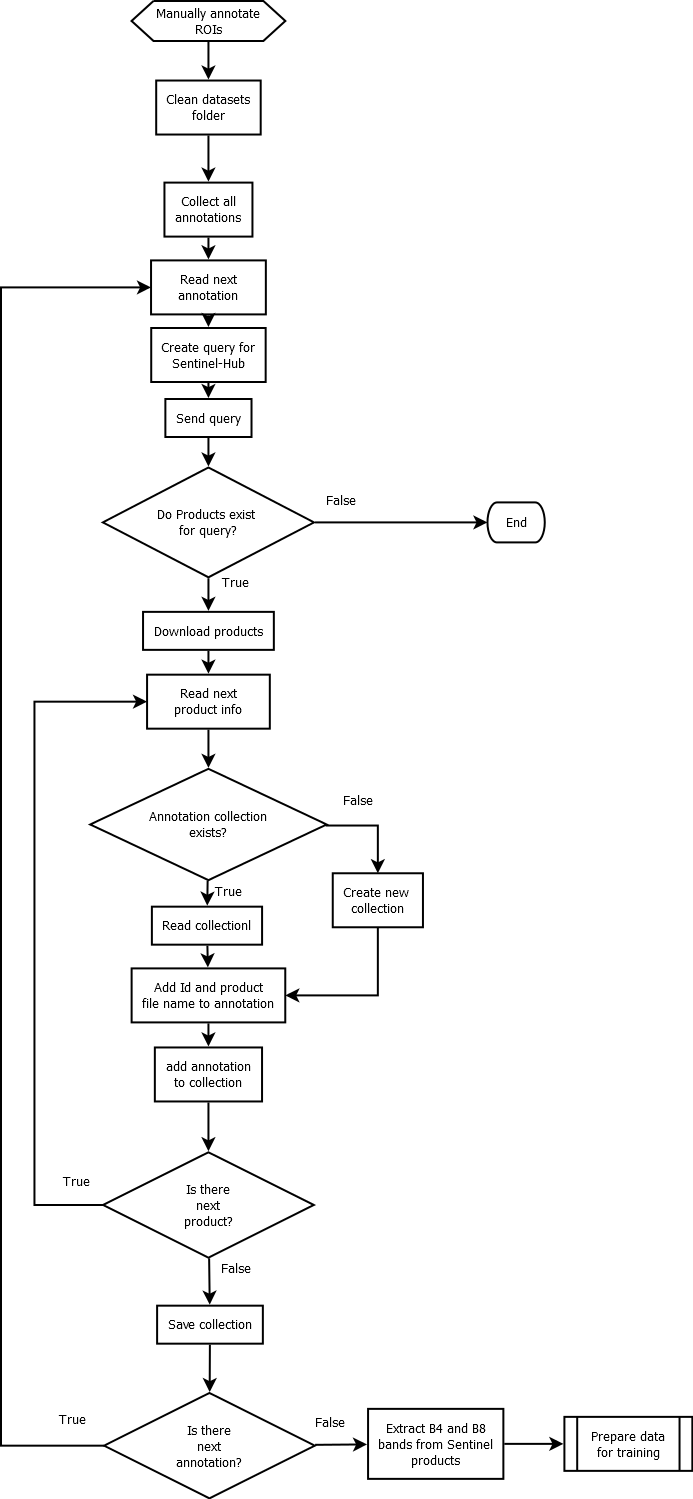
\includegraphics[height=\textheight]{pics/get-products.png}
  \caption{Ablaufdiagramm der Beschaffung der Sentinelprodukte}
  \label{fig:get-products}
\end{figure}

Der \textit{Copernicus Open Access Hub}\footnote{\url{https://scihub.copernicus.eu/}} ermöglicht freien und offenen Zugriff auf Sentinel-Produkte. Die Daten sind sowohl über eine grafische Oberfläche als auch über eine REST-API verfübar. Vorrausgesetzung für beide Optionen ist ein Account, der über die grafische Oberfläche erstellt werden kann.
\\\\
Die Nutzung der Schnittstelle erfolgt über die Python-Bibliothek \texttt{sentinelsat}\footnote{https://sentinelsat.readthedocs.io/en/stable}. Bei einer Anfrage müssen die GeoJSON-Dateien in WKT\footnote{WKT (Well-known text) ist eine Markup-Sprache zur Repräsentation von geometrischen Objekten auf Karten und räumlichen Referenzsystemen.} umgewandelt werden, was von der Bibliothek übernommen werden kann. Die WKT-Geometrie wird als \textit{footprint} (dt.: Fußabdruck) bezeichnet. Desweiteren wird der Plattformname statisch als `Sentinel-2' definiert, damit keine Produkte von den anderen Sentinelplattformen zurückgegeben werden. Der Suchzeitraum wird aus der jeweiligen GeoJSON-Datei übernommen. Sollten für die Suchanfragen keine Produkte existieren, wird die Anwendung beendet, da es keine Basis gibt, auf der das Netzwerk trainiert werden kann. Eventuell muss bei so einem Fall der Zeitraum erweitert und Prozess wiederholt werden. Bei vorhandenen Produkten lädt das Skript diese herunter. Die Produkte werden in einem komprimierten Format geliefert und enthalten neben zusätzlichen Informationen, Banddaten in separaten Dateien im JPEG2000-Format\footnote{JPEG 2000 genau wie GeoTIFF ist ein Bildformat in dem auch Metadaten abgelegt werden können. So sind Pixel geografischen Koordinaten zuordbar.}.
\\\\
Für jedes Produkt, das zur aktuellen Annotation gehört, wird ein neuer Eintrag zu einer \textit{FeatureCollection} hinzugefügt. Zusätzlich wird eine \textit{UUID} (Universally Unique Identifier) generiert und zusammen mit dem Dateinamen der Produktes in den Metadaten gespeichert. Für die spätere Entwicklung sind die Annotationen leichter zu finden und bearbeitbar. Außerdem bleiben dadurch die Originaldaten unberührt. Dieser Schritt wird für jede vorhandene Annotationsdatei wiederholt. Anschließend werden die Bilddateien für B4 und B8 aus dem Produkt extrahiert.

\section{Aufbereitung der Sentineldaten}
\chapter{Experimente}\label{chap:experiments}

Nach der Beschreibung des Konzept und Verlauf des Python-Skripts geht dieses Kapitel auf die wichtigsten Trainingsdurchläufe ein und diskutiert die Ergebnisse. 
\\\\
Es wurden iterativ Trainingprozeduren durchgeführt mit jeweils unterschiedlichen Konfiguration, wie um vorherigen Kapitel gezeigt, und miteinander verglichen. Die genauen Konfigurationen werden bei den einzelnen Experimenten angeführt. Die Experimente liefen auf einem Rechner mit NVIDIA TITAN Xp 12 GB VRAM Grafikkarte, Intel i7-7800X CPU und 32 GB RAM. Da diese Arbeit zeitlich begrenzt ist, wurden die Experimente auf max. 100 Epochen begrenzt, was die durchschnittliche Laufzeit auf etwa drei bis vier Stunden je Experiment bringt. Diese Beschränkung wirkt ebenfalls Overfitting entgegen, da nicht ausreichend Zeit hat, um sich auf den Trainingsdatensatz "`einzugewöhnen"'.
\\\\
Es wurden drei unterschiedliche Datensätze aus den Sentinelprodukten erzeugt. 
\begin{enumerate}
	\item Der originale unaugmentierte Datensatz enthält insgesamt jeweils zwölf Bilder und Masken\footnote{Trainingsanteil: 7, Validationsanteil: 2, Testanteil: 3} und dient als Basis für das Ausgangsexperiment. 
	\item Der augmentierte Datansatz (s. Kapitel \ref{sec:augmentation}) enthält 1291 Dateien und Masken\footnote{Trainingsanteil: 825, Validationsanteil: 207, Testanteil: 259}. Nachdem die zufällige Ausschnitte produziert wurden, kam es vor, dass einige Masken keinen \textit{RoI}-Anteil enthielten. Diese Masken und auch die zugehörigen Bilddateien wurden verworfen und weicht deswegen von der eigentlichen Größe von 1296 Elementen\footnote{Die zwölf ursprünglichen Dateien multipliziert mit dem Data Augmentation-Faktor von 108.} ab.
	\item In einem dritten Datensatz wurden Ausschnitte benutzt, deren Bildgrenzen sich an den äußersten Punkten der Masken befinden (s. Abb. \ref{fig:example-overfitting}). Dieser Datensatz wurde ausschließlich mittels Rotationen erweitert und enthält 144 Elemente\footnote{Trainingsanteil: 92, Validationsanteil: 23, Testanteil: 29}. 
\end{enumerate}
\noindent

\section{Training mit Rohdaten}\label{sub:sub:sec:experiment-1}

\begin{lstlisting}[language=python,caption={Konfiguration für Experimente 1},captionpos=b]
class CropDiseaseConfig(Config):
    BACKBONE = "resnet50"
    IMAGE_MAX_DIM = 128
    IMAGE_MIN_DIM = 128
    IMAGE_RESIZE_MODE = "square"
    IMAGES_PER_GPU = 4
    LEARNING_RATE = 0.001
    NUM_CLASSES = 1 + 1
    RPN_ANCHOR_SCALES = (8, 16, 32, 64, 128)
    STEPS_PER_EPOCH = 23
    USE_MINI_MASK = False
\end{lstlisting}
\noindent
Zuerst wurden ein Modell auf Datensatz 1 und alle Schichten des Modells wurden trainiert. Diese Experimente sollen zeigen, wie ein zu kleiner Datensatz sich auswirken kann.

\begin{figure}[ht]
	\centering
    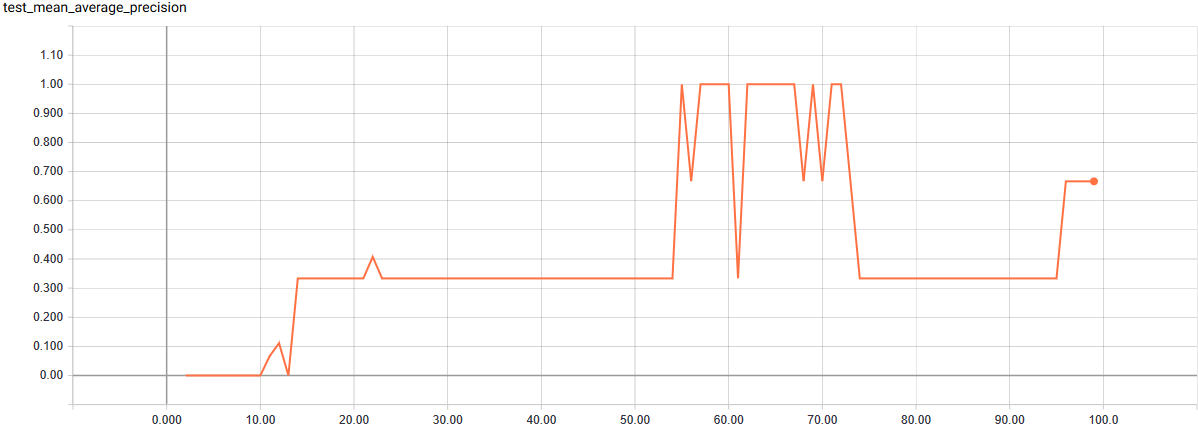
\includegraphics[width=.7\textwidth]{pics/map-1.PNG}
    \caption{\textit{mAP}-Graph von Experiment 1, X-Achse: Epochennummer, Y-Achse: \textit{mAP}-Werte}
    \label{fig:map-1}
\end{figure}
\begin{figure}[ht]
	\centering
    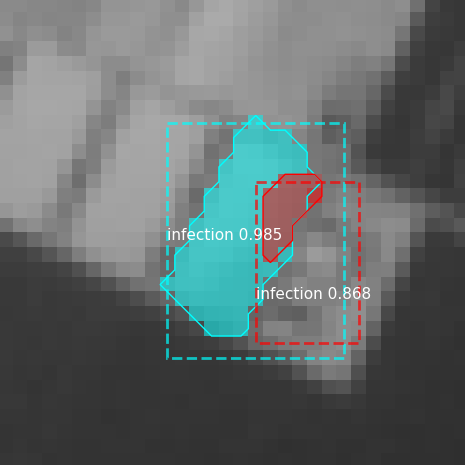
\includegraphics[height=3.5cm]{pics/pred-1-1.png}
    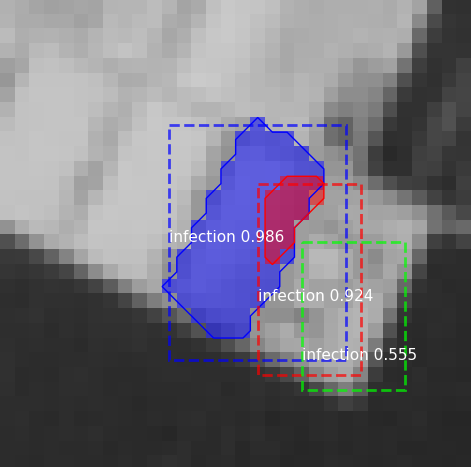
\includegraphics[height=3.5cm]{pics/pred-1-2.png}
    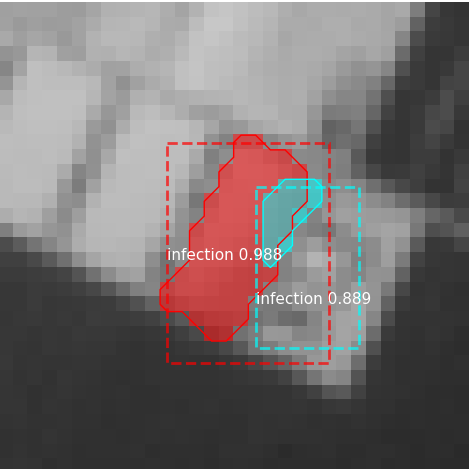
\includegraphics[height=3.5cm]{pics/pred-1-3.png}
    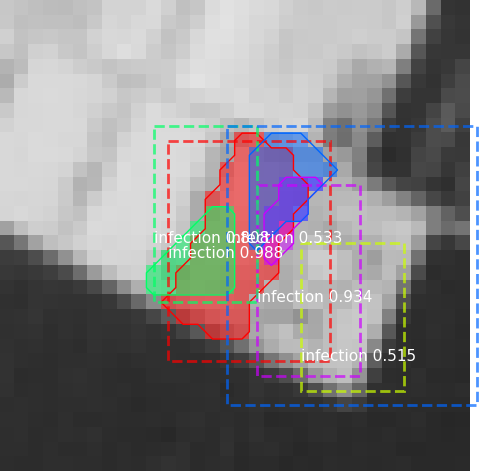
\includegraphics[height=3.5cm]{pics/pred-1-4.png}
    \caption[Beispielvorhersagen Experiment 1]{Beispielvorhersagen anhand der Gewichte von Epoche 55}
    \label{fig:pred-1}
\end{figure}
\noindent
Man sieht, dass das Modell während des Trainings unterdurchschnittliche Ergebnisse erzielt, was wenig überraschend ist, da der Datensatz sehr klein ist. Da nach jeder Epoche die Gewichte zwischengespeichert werden, können diese einzeln geladen werden. So wurde für eine Detektion ein Modell mit den Gewichten der 55. Epoche initialisiert, da sich hier der \textit{mAP}-Wert auf dem Maximalwert befindet. Die Bilder in Abb. \ref{fig:pred-1} entstammen einem fremden Datensatz, ähneln aber in den Grundcharakteristika dem eigentlichen Datensatz 1. Zum Beispiel ist das Zielfeld ähnlich ausgerichtet und zentriert. Man sieht, dass sich die berechneten Masken relativ genau auf das Zielfeld eingrenzen. Jedoch sind die erzeugten Bounding-Boxen und passen nicht zu den entsprechenden Masken, falls eine Maske erkannt wurde. Auch wurden mehrere Objektinstanzen erkannt, wobei eine einzige Instanz detektiert werden sollte. Werden die Bilder in Abb. \ref{fig:pred-1} nun vertikal gespiegelt und in das Netzwerk gegeben, erzeugt das Modell keine Masken, obwohl lediglich die Ausrichtung verändert wurde. Das ist ein Hinweis auf Overfitting, da das neuronale Netz minimale Änderungen nicht mehr erkennt.

\section{Datensatzerweiterung durch Rotation}\label{sub:sub:sec:experiment-2}

\begin{lstlisting}[language=python,caption={Konfiguration für Experiment 2},captionpos=b]
class CropDiseaseConfig(Config):
    BACKBONE = "resnet50"
    IMAGE_MAX_DIM = 128
    IMAGE_MIN_DIM = 128
    IMAGE_RESIZE_MODE = "square"
    IMAGES_PER_GPU = 4
    LEARNING_RATE = 0.001
    NUM_CLASSES = 1 + 1
    RPN_ANCHOR_SCALES = (8, 16, 32, 64, 128)
    STEPS_PER_EPOCH = 206
    USE_MINI_MASK = False
\end{lstlisting}
\noindent
Bei diesem Experiment wurde ein Modell Datensatz 3 und alle Schichten des Modells trainiert. Die Konfiguration bleibt unverändert, jedoch ist hier der augementierte Datensatz vergleichweise größer.

\begin{figure}[ht]
	\centering
    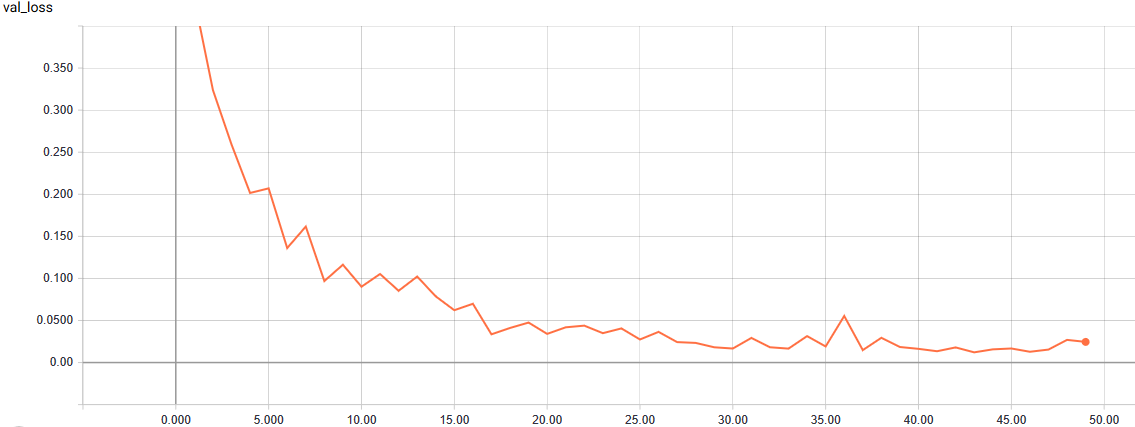
\includegraphics[width=.7\textwidth]{pics/val-loss-2.PNG}
    \caption{\textit{loss}-Graph von Experiment 2, X-Achse: Epochennummer, Y-Achse: \textit{loss}-Werte}
    \label{fig:val-loss-2}
\end{figure}

\begin{figure}[ht]
	\centering
    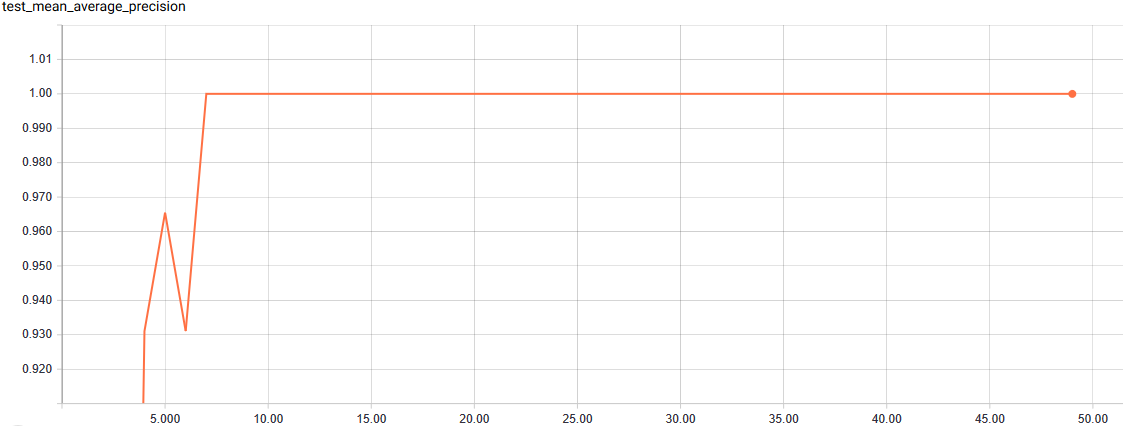
\includegraphics[width=.7\textwidth]{pics/map-2.PNG}
    \caption{\textit{mAP}-Graph von Experiment 2, X-Achse: Epochennummer, Y-Achse: \textit{mAP}-Werte}
    \label{fig:map-2}
\end{figure}

\begin{figure}[ht]
  \centering
  \begin{minipage}[c]{.3\textwidth}
  \centering
  
\includegraphics[height=2cm]{pics/roi-2-1.png}
  \\ \vspace{.25cm}
  
\includegraphics[height=3cm]{pics/roi-2-2.png}
  \\ \vspace{.25cm}
  
\includegraphics[height=3cm]{pics/roi-2-3.png}
  \\ \vspace{.25cm}
  
\includegraphics[height=3cm]{pics/roi-2-4.png}
  \end{minipage}
  \begin{minipage}[c]{.3\textwidth}
  \centering
  
\includegraphics[height=2cm]{pics/mask-2-1.png}
  \\ \vspace{.25cm}
  
\includegraphics[height=3cm]{pics/mask-2-2.png}
  \\ \vspace{.25cm}
  
\includegraphics[height=3cm]{pics/mask-2-3.png}
  \\ \vspace{.25cm}
  
\includegraphics[height=3cm]{pics/mask-2-4.png}
  \end{minipage}
  \begin{minipage}[c]{.3\textwidth}
  \centering
  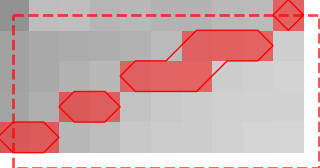
\includegraphics[height=2cm]{pics/pred-2-1.png}
  \\ \vspace{.25cm}
  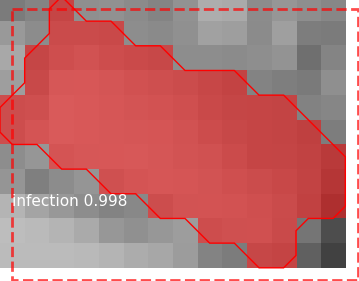
\includegraphics[height=3cm]{pics/pred-2-2.png}
  \\ \vspace{.25cm}
  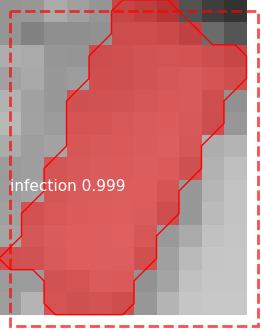
\includegraphics[height=3cm]{pics/pred-2-3.png}
  \\ \vspace{.25cm}
  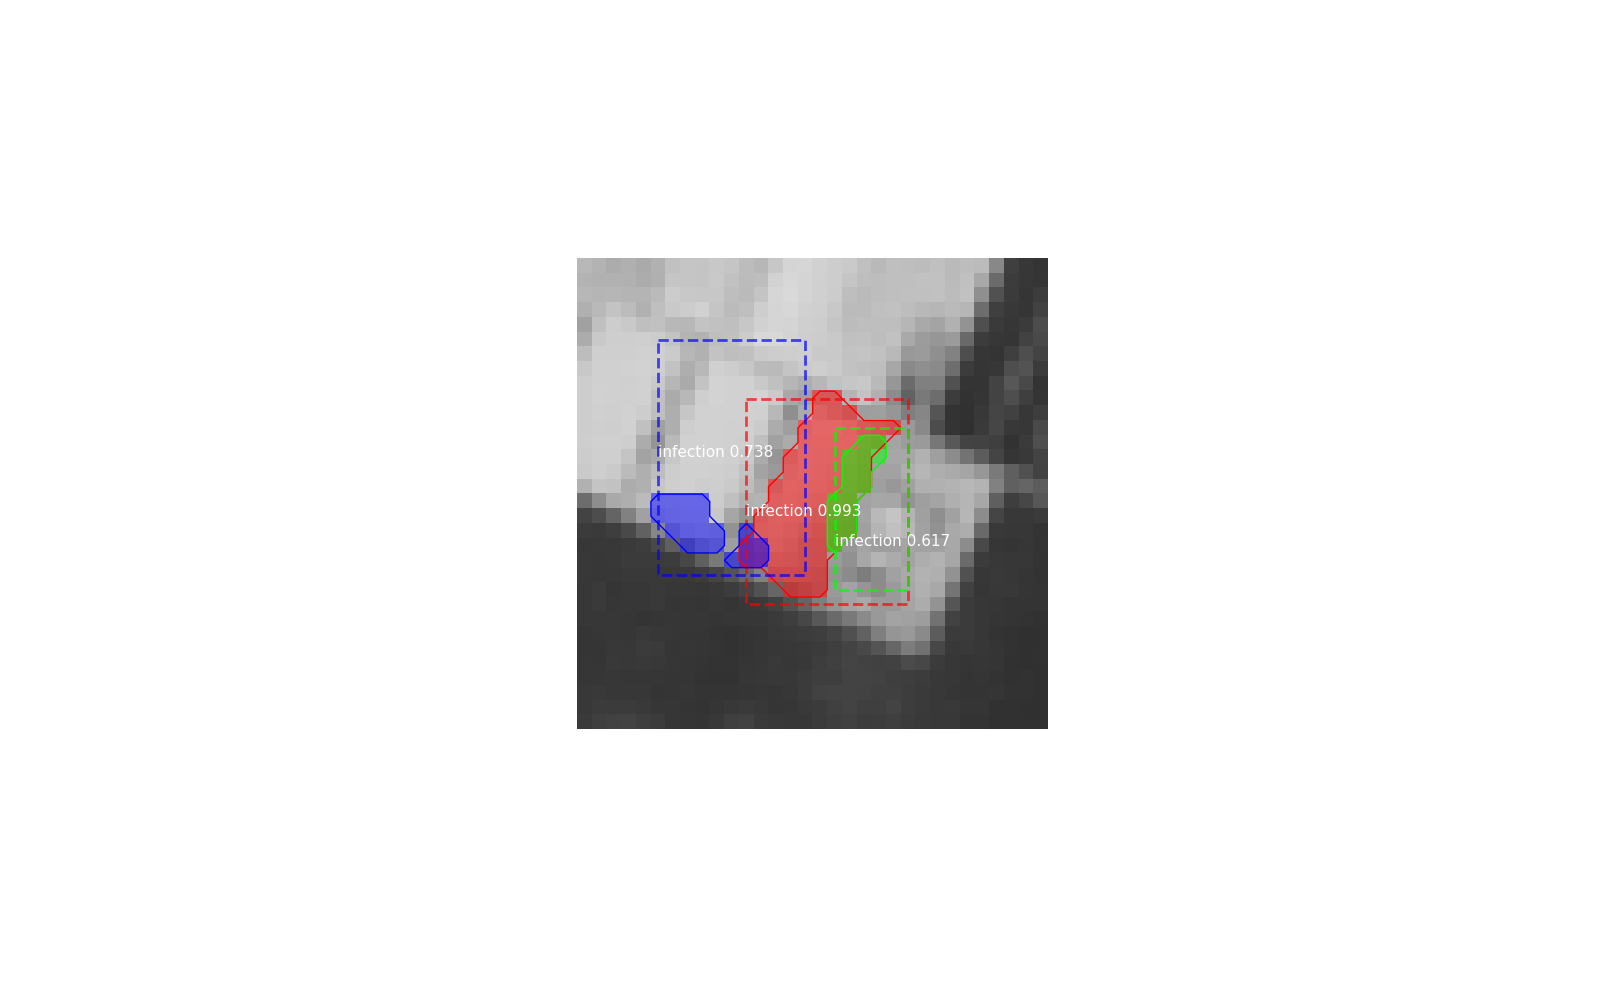
\includegraphics[height=3cm]{pics/pred-2-4.png}
  \end{minipage}

  \caption[Beispielvorhersagen Experiment 2]{Beispielvorhersagen anhand der Gewichte von Epoche 37, links: Ausgangsbild, mitte: Maske, rechts: Detektion}
  \label{fig:pred-2}
\end{figure}
\noindent
Die \textit{mAP}-Kurve konvergiert ab Epoche 7 gegen $1$ und verweilt dort für den Rest des Trainings. Dagegen sinken die $loss$-Werte weiterhin und nähern sich ab Epoche 37 $0$ an. Daher wurde die Gewichte dieser Epoche näher untersucht. Abb. \ref{fig:pred-2} zeigt, dass das Modell resistenter gegenüber Rotationen ist. Nichtsdestotrotz reagiert das Modell empfindlich auf Veränderungen wie zum Beispiel ein größerer Ausschnitt oder Translationen (s. unterste Reihe in Abb. \ref{fig:pred-2}). Daraus ergibt sich, dass das Modell nicht allgemein einsetzbar ist und die Daten durch weitere Augmentationen randomisiert werden müssen.
\newpage
\section{Data Augmention und Regularization}\label{sec:experiment-3}

\begin{lstlisting}[language=python,caption={Konfiguration für Experiment 3},captionpos=b,label=lst:experiment-3]
class CropDiseaseConfig(Config):
    BACKBONE = "resnet50"
    IMAGE_MAX_DIM = 128
    IMAGE_MIN_DIM = 128
    IMAGE_RESIZE_MODE = "square"
    IMAGES_PER_GPU = 4
    LEARNING_RATE = 0.001
    NUM_CLASSES = 1 + 1
    RPN_ANCHOR_SCALES = (8, 16, 32, 64, 128)
    STEPS_PER_EPOCH = 3
    USE_MINI_MASK = False
    WEIGHT_DECAY = 0.0001 # Orange, Dunkelblau, Rot
    WEIGHT_DECAY = 0.001 # Pink
    WEIGHT_DECAY = 0.01 # Hellblau
\end{lstlisting}
\noindent
Diese Sektion vergleicht mehrere Traingsläufe direkt miteinander. Zur simpleren Kommunikation werden die einzelnen Durchläufe mit den Farben betitelt, wie sie in den Graphen \ref{fig:val-loss-3} und \ref{fig:map-3} (Orange, Rot, Pink, Hell- und Dunkelblau) repräsentiert sind. Die verschiedenen \texttt{WEIGHT\_DECAY}-Werte in Listing \ref{lst:experiment-3} sind in den entsprechenden Modellkonfigurationen zu verwenden, wie sie in den Kommentaren benannt sind, wobei der Wert für die orangene, rote und dunkelblaue Konfigurationen implizit in der Basisklasse \texttt{Config} definiert ist. Die pinke und hellblaue Konfiguration soll den Einfluss von L2 Regularization zeigen. Alle Modelle bis auf das orangene wurden auf Grundlage von Datensatz 2 trainiert. Aus Gründen, die später erklärt werden, wurde für das orangene Modell ein Datensatz kreiert, das sich auf die kleine Zone innerhalb des Feldes mit der stärkeren Infektionskonzentration beschränkt. Der \textit{head} des dunkelblauen Netzwerk wurde trainiert, während alle Schichten der restlichen Modelle trainiert wurden.

\begin{figure}[ht]
	\centering
    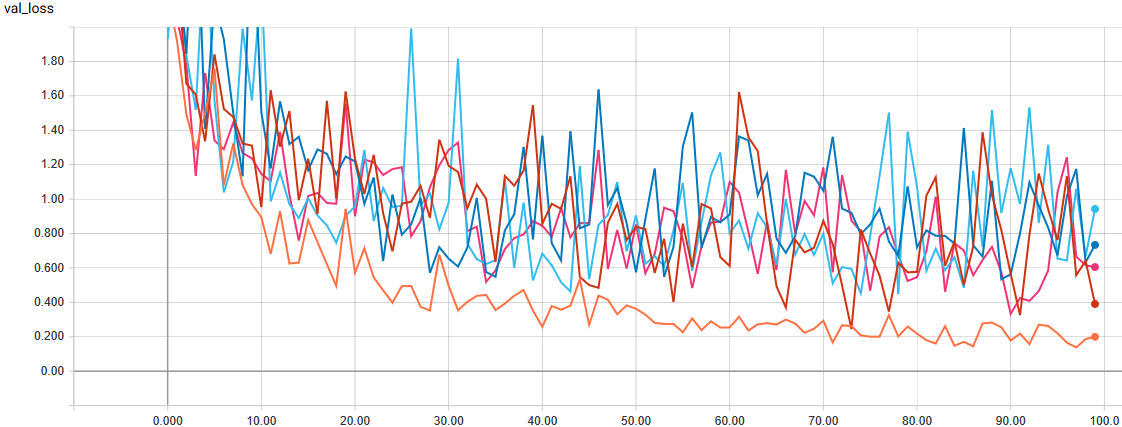
\includegraphics[width=.7\textwidth]{pics/val-loss-3.PNG}
    \caption{\textit{loss}-Graph von Experiment 2, X-Achse: Epochennummer, Y-Achse: \textit{loss}-Werte}
    \label{fig:val-loss-3}
\end{figure}

\begin{figure}[ht]
	\centering
    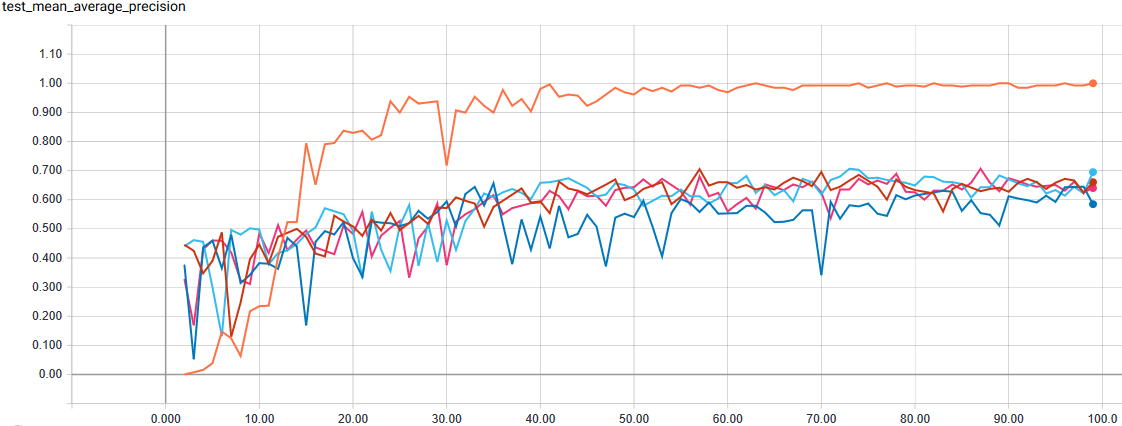
\includegraphics[width=.7\textwidth]{pics/map-3.PNG}
    \caption{\textit{mAP}-Graph von Experiment 2, X-Achse: Epochennummer, Y-Achse: \textit{mAP}-Werte}
    \label{fig:map-3}
\end{figure}

\begin{figure}[H]
  \centering
  \begin{minipage}[c]{.3\textwidth}
  \centering
  
\includegraphics[height=3cm]{pics/roi-3-2.png}
  \\ \vspace{.25cm}
  
\includegraphics[height=3cm]{pics/roi-3-3.png}
  \\ \vspace{.25cm}
  
\includegraphics[height=3cm]{pics/roi-3-4.png}
  \\ \vspace{.25cm}
  
\includegraphics[height=3cm]{pics/roi-3-5.png}
  \\ \vspace{.25cm}
  
\includegraphics[height=3cm]{pics/roi-3-1.png}
  \end{minipage}
  \begin{minipage}[c]{.3\textwidth}
  \centering
  
\includegraphics[height=3cm]{pics/mask-3-2.png}
  \\ \vspace{.25cm}
  
\includegraphics[height=3cm]{pics/mask-3-3.png}
  \\ \vspace{.25cm}
  
\includegraphics[height=3cm]{pics/mask-3-4.png}
  \\ \vspace{.25cm}
  
\includegraphics[height=3cm]{pics/mask-3-5.png}
  \\ \vspace{.25cm}
  
\includegraphics[height=3cm]{pics/mask-3-1.png}
  \end{minipage}
  \begin{minipage}[c]{.3\textwidth}
  \centering
  \includegraphics[height=3cm]{pics/pred-3-2.png}
  \\ \vspace{.25cm}
  \includegraphics[height=3cm]{pics/pred-3-3.png}
  \\ \vspace{.25cm}
  \includegraphics[height=3cm]{pics/pred-3-4.png}
  \\ \vspace{.25cm}
  \includegraphics[height=3cm]{pics/pred-3-5.png}
  \\ \vspace{.25cm}
  \includegraphics[height=3cm]{pics/pred-3-1.png}
  \end{minipage}

  \caption[Beispielvorhersagen Experiment 2]{Beispielvorhersagen verschiedener Modelle, v.l.n.r.: Ausgangsbild, Masken, Vorhersage, v.o.n.u.: Vorhersagen von dunkelblau, rot, hellblau, pink, orange}
  \label{fig:pred-3}
\end{figure}
\noindent
Für auf Datensatz 3 trainierten Modelle (jeweils Epoche 100) zeichnen sich in  Abb. \ref{fig:val-loss-3} starke Schwankungen ab und kein Modell überschreitet $mAP>0.7$. Die Vorhersagen in den oberen vier Reihen in Abb. \ref{fig:pred-3} stimmen zum großen Teil mit den Masken überein. Weitere hier nicht aufgeführte Vorhersagen zeigen ähnliche Ergebnisse. Es kommt vor, dass die kleine Zielregion vorhergesagt wird, obwohl die entsprechende binäre Maske die große \textit{RoI} repräsentiert, so ähnlich wie es in der unteren Reihe zu sehen ist. Dieses Verhalten erklärt die schlechten \textit{mAP}-Kurven und die Schwankungen. Da die Detektion nicht mit dem erwarteten Ergebnis übereinstimmt und daher der berechnete Fehler höher ist, obwohl die Detektion eigentlich korrekt ist, da sich beide genutzten \textit{RoIs} geografisch schneiden. Durch den Fehler ist die Korrektur der Gewichte entsprechend größer. Um die Annahme zu bekräftigen, wurde ein Modell (orange) auf dem speziellen Datensatz trainiert. Im Vergleich zu den anderen Kurven konvergiert die orangene \textit{loss}-Kurve gegen $0$ bzw. die orangene \textit{mAP}-Kurve gegen $1$. Wäre mehrere unterschiedliche \textit{RoIs} vorhanden, die sich nicht schneiden, würde der Einfluss sich nicht bemerkbar machen. Was hier jedoch nicht der Fall ist, da beide \textit{RoIs} jeweils etwa die Hälfte des Datensatzes ausmachen.
\\\\
Es ist zu sehen, dass die \textit{Ridge Regression} (hellblau und pink) keinen merkbaren Einfluss auf das Training haben, weil einen ähnlichen Verlauf wie die dunkelblaue und rote Kurven haben. Im Gegensatz dazu zeigt die \textit{Data Augmentation} positive Ergebnisse (s. Abb. \ref{fig:pred-3}) und alle Modelle sind deutlich robuster gegenüber manipulierten Bildern. Jedoch schlagen die Detektionen bei größeren Ausschnitten fehl oder geben sinnlose Resultate zurück. Weiterhin sei erwähnt, dass das Modell, dessen \textit{head} trainiert wurde, von allen hier erwähnten Modellen am schlechtesten abschneidet und es zumindest nicht hilfreich ist, nur die oberen Schichten zu trainieren.

\chapter{Ergebnisdiskussion}

Ergebnisse zeigen, dass Mask R-CNN ein potentielles Werkzeug ist, um Landwirte bei der Kontrolle ihrer Felder zu unterstützen. Die implementierte Anwendung lädt automatisch Sentinelprodukte herunter, extrahiert die gefragten Bildregionen und berechnet daraus einen Gesundheitsindex der Flächen. Ein konfiguriertes Mask R-CNN-Modell analysiert die Indexwerte auf Muster, die mit Krankheiten korrelieren könnten. 
\\\\
Das Ziel der Arbeit eine Vielzahl von Krankheiten zu analysieren und zu identifizieren, konnte nicht erreicht werden, da hier nur eine Region zur Verfügung stand. Aufgrund dessen wurden wie erwartet bei ersten Experimenten Modelle trainiert, die Overfitting aufwiesen. Nichtsdestotrotz half Data Augmentation, die Größe des Datensatzes zu erweitern und Variationen in Form und Ausrichtung der Ausgangsfläche zu erzeugen. Dadurch konnte ein Modell trainiert werden, dass Resistenz gegenüber Overfitting aufwies. Der Einsatz von Data Augmentation ist ebenfalls sinnvoll sollte kein Overfitting vorliegen. Ausbreitungen von Infektionen sind willkürlich und folgen keinen bestimmten geometrischen Mustern. Data Augmentation hilft durch künstliche Randomisierungen ein Modell darauf vorzubereiten.
\\\\
Jedoch zeigten die oft bei Overfitting verwandte Ridge Regression keinerlei Auswirkung. Wenn einige ausgewählte Neuronen-Schichten trainiert wurden, verschlechterte sich die allgemeine Performanz. Deswegen sind L2 Regularization und Training ausgewählter Schichten in weiteren Untersuchungen, die nur mit hier untersuchten Felddaten arbeiten, nicht zu empfehlen. Es ist aber nicht abzusehen, wie sich das Modell verhalten wird, wenn 
\\\\
Weiterhin wurde die Vermutung aufgestellt, dass die \textit{RoIs} negative Einflüsse auf die Bewertung des Trainings haben, da eine Region von der zweiten Region umschlossen wird. Ein Modell, dass auf Grundlage einer Region trainiert wurde, erzielt bessere \textit{mAP}-Werte und bestärkt dadurch diese Annahme. Weitere Forschungen sollten den Datensatz, um andere Felddaten erweitern. Durch eine größere Vielfalt können solche Einflüsse ignoriert werden, da der Effekt dadurch entsteht einen minimalen Einfluss bei der Fehlerberechnung hat. Ebenso sind weitere Daten notwendig, um den produktiven Einsatz zu bestätigen.

\chapter{Zusammenfassung und Fazit}\label{chap:summary}

Ziel der Arbeit war es ein heuristisches Modell zu trainieren, das in der Lage ist, anhand von Satellitenaufnahmen infizierte Agrarfläche zu analysieren und eventuelle Krankheitsbefälle zu erkennen. 
\\\\
Das Skript, das im Rahmen dieser Abschlussarbeit entwickelt wurde, fasst mehrere Disziplinen zusammen. Deswegen war eine ausführliche Ausarbeitung in Thematiken wie pflanzliche Biologie, Lichtspektren, geografische Referenzsysteme und künstliche neuronale Netze notwendig, um ein tiefgehendes Verständnis für die Problematik und für den Zusammenhang zwischen Lichtreflexion einer Pflanze und deren Stress- bzw. Gesundheitsstatus zu erlangen. Gesunde bzw. gestresste Pflanzen besitzen einen hohen bzw. niedrigen Chlorophyllspiegel und dieser sorgt dafür, dass die Pflanzen im nahen Infrarotbereich stärker bzw. schwächer zurückstrahlen. Diese Reflexionen können über Sentinel-2-Multispektralaufnahmen gemessen werden und daraus lässt sich ein Vitalitätsindikator NDVI berechnen.
\\\\
Die berechneten NDVI-Werte sollten in einem bewachten Lernverfahren ein neuronales Netz trainieren. Jedoch war früh ersichtlich, dass historische Daten rar sind und dadurch war auch mit Overfitting zu rechnen. Es wurden mehrere Methoden untersucht, um einem Overfitting entgegen zu wirken wie etwa Vergrößerung des Datensatzes durch Data Augmentation oder Hinzufügen eines weiteren Hyperparameters durch Ridge Regression. 
\\\\
Als zu trainierendes KNN wurde die Mask R-CNN-Implementierung ausgewählt, da sie unter anderem eine hohe Robustheit aufweist und Objektinstanzen auf Pixelebene klassifizieren kann. 
\\\\
Nachdem Modell und Methoden zur Modellevaluation und gegen Overfitting ausgesucht wurden, wurde ein Prozessablauf ausgearbeitet, der automatisch Sentinelprodukte in einem vorherdefinierten Zeitraum und einer geographischen Umgebung herunterlädt, verarbeitet und das Training bzw. Detektionen ausführt. Darauf wurde der konzeptionierte Prozess implementiert und das Modell durch anschließende Experimente evaluiert.
\\\\
Die Experimente zeigten positive Ergebnisse durch Data Augmentation. Die anfangs trainierten Modelle ohne Data Augmentation lieferten bei leichten Veränderungen der bekannten Daten wie Rotationen oder Spiegelungen keine brauchbaren Resultate. Währenddessen sind mit Data Augmentation trainierte Modelle dagegen resistenter. Allerdings zeigte die L2 Regularization keinerlei Auswirkung.
\\\\
Es ist möglich, mit der Mask R-CNN-Architektur ein Modell trainieren zu können, das zuverlässig die hier untersuchten Krankheiten erkennt und eingrenzen kann. Fremde Pathogene werden von diesem Modell wahrscheinlich nicht erkannt, da jede Krankheit und folglich die Auswirkung auf die Pflanze unterschiedlich ist. Es sind weitere Untersuchungen mit zusätzlichen Daten notwendig, die zum Abschluss der Arbeit nicht verfügbar waren. Zum einen, um die in Kapitel \ref{sec:experiment-3} beschriebenen Schwankungen ausgleichen zu können. Zum anderen, um einen Datensatz zu haben, der ein fremdes mit der selben Krankheit infiziertes Feld enthält, der dazu dient, die hier erlangten Ergebnisse zu bestätigen. 
\\\\
Gegen Ende der Ausarbeitung gaben Mitarbeiter des CREA bekannt, im Laufe des Jahres 2019 weitere Felder auf Infektionen untersuchen zu wollen und diese entsprechend weiterzuleiten. Auf Basis dieser Daten können zukünftig weitere Experimente definiert, durchgeführt und evaluiert werden. Um mehr Satellitendaten in einem Zeitraum zu erhalten, können andere Satelliten wie etwa SPOT-5 angesprochen werden. Wichtig hierbei ist, dass die Satelliten eine gleiche oder höhere räumliche Auflösung besitzen und Aufnahmen im roten und nahen infraroten Bereich machen können. 


%\printbibliography
\bibliographystyle{babplain-lf}
\bibliography{literature}

% ----- Abbildungen ----- %
\listoffigures


% ----- Tabellen----- %
\listoftables

	
% ----- Listings ----- %

\chapter*{Erklärung}
\addcontentsline{toc}{chapter}{Erklärung}

Ich versichere, dass ich die vorliegende Arbeit selbstständig und nur unter Verwendung der angegebenen Quellen und Hilfsmittel angefertigt habe, insbesondere sind wörtliche oder sinngemäße Zitate als solche gekennzeichnet. Mir ist bekannt, dass Zuwiderhandlung auch nachträglich zur Aberkennung des Abschlusses führen kann.\\\\
Ich versichere, dass das elektronische Exemplar mit den gedruckten Exemplaren übereinstimmt.
\\\\\\
Ort:\hspace{3cm}Datum:\hspace{3cm}Unterschrift:

\end{document}